\documentclass[11pt]{amsart}
\usepackage{amsmath,amssymb,amsthm}
\usepackage[margin=1.1in]{geometry}
\usepackage{graphicx}
\usepackage{hyperref}
\setlength{\emergencystretch}{3em}

\newtheorem{theorem}{Theorem}
\newtheorem{lemma}{Lemma}[section]
\newtheorem{corollary}[lemma]{Corollary}
\newtheorem{conjecture}[theorem]{Conjecture}
\theoremstyle{remark}
\newtheorem{remark}[lemma]{Remark}

\newcommand{\E}{\mathbb{E}}
\newcommand{\Prob}{\mathbb{P}}
\newcommand{\Z}{\mathbb{Z}}

\title[The distribution of the theta-function sum $S(p)$]{The distribution of the theta-function sum $S(p)$:\\ limit law, character expansion, sharp tails and extreme values}
\author{Samson Fraser}
\email{samsonmfraser@gmail.com}
\date{October 2026}

\begin{document}

\begin{abstract}
For a prime $p$ let $S(p)=\sum_{h,j=1}^{p-1}(-1)^{j+1+\lfloor hj/p\rfloor}$, a sum studied by Berndt, Bhat, Meyer, Xie and Zaharescu, and put $X_p=S(p)/p-\frac12\log p$. We prove that $X_p$ has a limiting distribution $\nu$ over the primes, and that the moments of $X_p$ converge to those of $\nu$. The law $\nu$ is symmetric about the constant $c_0=0.2399\ldots$. We express $\nu$ as an explicit series over odd Dirichlet characters, with coefficients given by $L(1,\chi)^2$ and an Euler product. This gives an exact formula for its variance, $\sigma^2\approx0.39237$, and closed forms for the limiting means of $X_p$ in residue classes; for example $c_0(3;\pm1)=c_0\pm\frac{\sqrt3\pi}{16}\prod_{\ell\equiv5\,(6)}(1+\frac2{(\ell-1)^2})$. The tails of $\nu$ are $\exp(-\exp((1+o(1))\sqrt{t/\kappa_H}))$ with $\kappa_H=2e^\gamma/\pi^2$. With the same constant, we show unconditionally and effectively that $X_p-c_0=\Omega_\pm((\log\log p)^2)$. Together these suggest $\limsup_p\pm(X_p-c_0)/(\log\log p)^2=\kappa_H$, of which we prove the lower bound. None of the results uses bounds for short Kloosterman sums. This is an AI-generated draft, not yet checked by a human expert; it relies on the asymptotic formula of an unrefereed companion paper.
\end{abstract}

\maketitle

\section{Introduction}

For an odd prime $p$, Berndt, Bhat, Meyer, Xie and Zaharescu \cite{BBMXZ} studied the sum
\[
S(p)=\sum_{h=1}^{p-1}\sum_{j=1}^{p-1}(-1)^{j+1+\lfloor hj/p\rfloor},
\]
which arises from a theta-function identity. They conjectured that $S(p)>0$, $S(p)>2p$ and $S(p)>3p$ beyond small thresholds, and that $C_1p<S(p)<C_2p^{1+\varepsilon}$ for large $p$. The companion paper~\cite{TS} proves the asymptotic formula
\begin{equation}\label{eq:B}
S(p)=\frac p2\log p+c_0p+\frac{4p}\pi R_K(p)+O\Big(\frac p{\log p}\Big),\qquad R_K(n)=\sum_{\substack{3\le k<K\\ k\ \mathrm{odd}}}\frac{F_k(n)}{k^2},
\end{equation}
for $\sqrt p(\log p)^4\le K\le p^{9/10}$, with $F_k(n)=\sum_{1\le t<k/2}\tan(\pi tn/k)$ and
\[
c_0=\frac{K_0}2+\frac{\log2}6+\frac3{\pi^2}\zeta'(2)=0.2399341036\ldots,\qquad K_0=\gamma+\log\frac4\pi
\]
\cite[Theorem~B(ii)]{TS}. Its proof uses Weil's bound for Kloosterman sums, and nothing deeper. This paper studies the fluctuating term
\[
X_p-c_0,\qquad X_p=\frac{S(p)}p-\frac12\log p,
\]
which by \eqref{eq:B} is $\frac4\pi R_K(p)+o(1)$.

\subsection*{Results}
Let $\nu$ be the law of $c_0+\frac4\pi R_\infty$, where $R_\infty$ is the $L^2$-limit of $R_K(x)$ for $x$ Haar-distributed on $\Omega=\prod_{\ell\ \mathrm{odd}}\Z_\ell^\times$ (Section~\ref{sec:G}).
\begin{itemize}
\item \emph{Limit law} (Theorem~\ref{thm:G}, Corollary~\ref{cor:moments}). The empirical distribution of $X_p$, $p\le x$, converges to $\nu$, together with all moments. The law $\nu$ is symmetric about $c_0$, and its support is unbounded in both directions. In residue classes the limits are the conditional laws, with means $c_0(q;r)$.
\item \emph{Character expansion} (Theorem~\ref{thm:J}). $R_\infty=\sum_\chi W(\chi)\chi$ over the odd primitive characters of odd conductor, with $W(\chi)$ explicit in $\tau(\chi)$, $L(1,\bar\chi)^2$ and an Euler product. Hence
\[
\sigma^2=\mathrm{Var}(\nu)=\frac1{\pi^2}\sum_\chi\frac{|2-\chi(2)|^4|L(1,\chi)|^4|E(\chi)|^2}{f_\chi\varphi(f_\chi)^2}\approx0.39237,
\]
where $E(\chi)$ is the Euler product of Section~\ref{sec:J}, and $c_0(q;r)$ is a finite sum over the characters of conductor dividing $q$.
\item \emph{Extreme values} (Theorem~\ref{thm:H}). Unconditionally and effectively, for every $\varepsilon>0$ and large $X$, at least $X^{1-o(1)}$ primes $p\in(X,2X]$ satisfy $X_p-c_0\ge(\kappa_H-\varepsilon)(\log\log p)^2$, and as many satisfy $X_p-c_0\le-(\kappa_H-\varepsilon)(\log\log p)^2$, where $\kappa_H=2e^\gamma/\pi^2=0.3609\ldots$.
\item \emph{Sharp tails} (Theorem~\ref{thm:I}). $\nu((c_0+t,\infty))=\nu((-\infty,c_0-t))=\exp(-\exp((1+o(1))\sqrt{t/\kappa_H}))$, and $\log\E e^{\theta(Z-c_0)}\sim\kappa_H\theta(\log\theta)^2$ for $Z\sim\nu$.
\item \emph{Further consequences.} The class means for smooth moduli have a two-term asymptotic, $c_0(Q_K;\pm1)=c_0\pm(\kappa_H\log K(\log K-\gamma-\log2+K_0)+C_Q+o(1))$ (Corollary~\ref{cor:smoothclass}). The density of primes with $\pm(X_p-c_0)>t$ is at least $\exp(-\exp((1+\varepsilon)\sqrt{t/\kappa_H}))$, uniformly up to $t\asymp(\log\log X)^2$ (Corollary~\ref{cor:unif}).
\end{itemize}
The tails and the extreme values carry the same constant $\kappa_H$. Comparing them leads to a precise conjecture (Conjecture~\ref{conj}): $\limsup\pm(X_p-c_0)/(\log\log p)^2=\kappa_H$. Theorem~\ref{thm:H} proves $\limsup\ge\kappa_H$ and $\liminf\le-\kappa_H$; the reverse inequalities are open. It is the analogue of the Montgomery--Vaughan conjecture for $L(1,\chi)$, and Theorem~\ref{thm:I} is the analogue of Granville and Soundararajan's theorem on the distribution of $L(1,\chi)$.

Earlier limit laws for cotangent and Dedekind sums \cite{Vardi,BD} average over all fractions $a/q$. By contrast, $S(p)$ involves one point per modulus. The numerical values of $c_0(q;r)$ were found in \cite{TS} by summing over $d\le8001$ and extrapolating; Theorem~\ref{thm:J} gives them in closed form.

\subsection*{What is used}
Standard references for the analytic tools are \cite{Dav,MV}. Besides \eqref{eq:B}, we use the elementary lemmas of \cite[Sections~4 and~9]{TS}, recalled in Section~\ref{sec:inputs}. We also use the prime number theorem in progressions (Siegel--Walfisz) for Theorem~\ref{thm:G}, and the Bombieri--Vinogradov theorem for the moments. Theorem~\ref{thm:H} uses Gallagher's prime number theorem and the Landau--Page lemma, and it avoids Siegel's theorem. No bounds for short Kloosterman sums are needed. In particular, none of the results depends on the Bourgain--Garaev bound, on which the lower half of the conjecture $S(p)>C_1p$ rests in~\cite{TS}.

The numbers quoted come from exact values of $S(p)$ for all primes $p\le5.5\cdot10^6$, from Haar samples of the model, and from the code \texttt{code/char\_expansion.py}, all in the repository that accompanies the main paper~\cite{TS}.

\section{Notation and inputs}\label{sec:inputs}

Results of \cite{TS} are cited by their numbers there; in particular (9.1) and (9.2) are equations of \cite{TS}. For odd $d\ge3$ put
\[
G_d(n)=\sum_{\substack{1\le j<d/2\\ (j,d)=1}}\tan\frac{\pi jn}d ,
\]
an odd function of $n\bmod d$. We use the following results of \cite{TS}.
\begin{itemize}
\item \emph{Theorem~B(ii)} is \eqref{eq:B}. In particular, for $p\in(X,2X]$ and $K_2=\sqrt{2X}(\log2X)^4$ we have $X_p-c_0=\frac4\pi R_{K_2}(p)+O(1/\log X)$.
\item \emph{Corollary~4.3.} (a) For odd $m\ge1$, $\frac m\pi(\log m+K_0)-\frac{7\pi}{72m}\le F_m(1)\le\frac m\pi(\log m+K_0)$. (b) For odd $k\ge3$ and every integer $r$, $|F_k(r)|\le F_k(1)\le\frac k\pi(\log k+K_0)$, and $F_k(-1)=-F_k(1)$.
\item \emph{Lemma~9.1.} $F_k(n)=\sum_{d\mid k,\,d\ge3}G_d(n)$ for odd $k$. Hence $R_K=\sum_{3\le d<K}w_d(K)G_d/d^2$, with $w_d(K)=\sum_{m\ \mathrm{odd},\,dm<K}m^{-2}\in[1,\pi^2/8]$. Also $R_{K_2}-R_{K_1}=\sum_dw_d(K_1,K_2)G_d/d^2$, with $0\le w_d(K_1,K_2)\le\min(\pi^2/8,2d/K_1)$.
\item \emph{Lemma~9.2.} Let $g\mid d$. (a) $A_{d,g}(s):=\frac gd\sum_{i<d/g}G_d(s+gi)=\sum_{j<d/2,(j,d)=1}\tan(\pi js/g)$. (b) $|A_{d,g}(s)|\le\frac{\tau(d)}\pi g(\log g+2)$ for $g\ge3$; in particular $|G_d(n)|\le\frac{\tau(d)}\pi d(\log d+2)$. (c) Let $A^*_{d,g}(s)$ be the average of $G_d(x)$ over the reduced residues $x\bmod d$ with $x\equiv s\pmod g$, $(s,g)=1$. Then $A^*_{d,1}=0$, and $|A^*_{d,g}(s)|\le C\tau(d)^2\lambda(d)g$ for $g\ge3$, where $\lambda(n)=(\log\log3n)(\log n+2)$.
\item \emph{The observation before (9.2).} If $x$ is uniform on the reduced residues modulo $k$ with $x\equiv r\pmod{(k,q)}$, then for $d\mid k$ the residue $x\bmod d$ is uniform on the reduced residues modulo $d$ with $x\equiv r\pmod{(d,q)}$.
\item \emph{The tangent identity} (proof of Lemma~9.2(a)). For odd $n$ and real $y$ avoiding poles, $\sum_{b<n}\tan(y+\pi b/n)=n\tan ny$.
\item \emph{(9.1).} If $L$ is a common multiple of $d,d'$ and $x$ is uniform on $(\Z/L\Z)^\times$, then $\E[G_d(x)G_{d'}(x)]=\E_s[A^*_{d,g}(s)A^*_{d',g}(s)]$ with $g=(d,d')$ and $s$ uniform on $(\Z/g\Z)^\times$. In particular the expectation vanishes when $g=1$.
\item \emph{Lemmas~9.3(b) and~9.4.} $\sum_{X<n\le2X}(R_{K_2}(n)-R_Y(n))^2\ll X(\log X)^{14}/Y$ for $3\le Y<K_2$.
\item \emph{Theorems~E and~F.} Theorem~E(i) says that $|X_p|\ll_A(\log\log p)^2$ for all $p\in(X,2X]$ outside a set of size $O_A(X(\log X)^{-A})$. Theorem~E(ii) says that $\sum_{X<p\le2X}(X_p-c_0)^2\ll X/\log X$, with an ineffective constant. Theorem~F gives the limiting mean $c_0(q;r)$ of $X_p$ over $p\equiv r\pmod q$, with $c_0(q;r)=c_0+\frac\pi2\sum_dA^*_{d,(d,q)}(r)/d^2$ by (9.2).
\end{itemize}

\section{The limiting distribution}\label{sec:G}

Let $\Omega=\prod_{\ell\ \text{odd prime}}\Z_\ell^\times$ with its Haar probability measure $\Prob$. For odd $k$ and $x\in\Omega$, $x\bmod k$ is a reduced residue, and we put $F_k(x)=F_k(n)$ and $G_d(x)=G_d(n)$ for any integer $n\equiv x\pmod{k}$, resp.\ $\pmod d$. For every odd $Q$, $x\bmod Q$ is uniformly distributed over $(\Z/Q\Z)^\times$. Hence expectations of functions of $x\bmod Q$ are the averages of \cite[Section~9]{TS}, and (9.1) holds under $\Prob$. As in \cite{TS}, $R_K(x)=\sum_{3\le k<K,\ k\text{ odd}}F_k(x)/k^2$. For a prime $p$ put
\[
X_p=\frac{S(p)}p-\frac12\log p .
\]

\begin{lemma}\label{lem:L2}
For $K\ge3$ let
\[
\mathcal E(K)=\sup_{K'>K}\E\big[(R_{K'}-R_K)^2\big].
\]
Then $\mathcal E(K)\to0$ as $K\to\infty$. Hence $R_K$ converges in $L^2(\Omega)$ to a limit $R_\infty$, with $\E[R_\infty]=0$ and
\[
\E[R_\infty^2]=\frac{\pi^4}{64}\sum_{d,d'\ge3\ \mathrm{odd}}\frac{\E[G_dG_{d'}]}{(dd')^2},
\]
the series being absolutely convergent.
\end{lemma}

\begin{proof}
By Lemma~9.1, $R_{K'}-R_K=\sum_{d<K'}w_d(K,K')G_d/d^2$ with $0\le w_d(K,K')\le\min(\pi^2/8,2d/K)$. By (9.1) and Lemma~9.2(c), $\E[G_dG_{d'}]=0$ unless $g=(d,d')\ge3$. In that case
\[
|\E[G_dG_{d'}]|\le C\tau(d)^2\tau(d')^2\lambda(d)\lambda(d')g^2,\qquad \lambda(n)=(\log\log3n)(\log n+2).
\]
Write $d=ga$ and $d'=ga'$, and drop the coprimality of $a,a'$; this gives the upper bound
\[
\E[(R_{K'}-R_K)^2]\le C\sum_{g\ge3}\sum_{a,a'\ge1}\min\Big(1,\frac{2ga}{K}\Big)\min\Big(1,\frac{2ga'}{K}\Big)\frac{\tau(ga)^2\tau(ga')^2\lambda(ga)\lambda(ga')}{g^2a^2a'^2}.
\]
Since $\tau(ga)\le\tau(g)\tau(a)$ and $\lambda(n)\ll n^{1/10}$, the summand is at most $\ll g^{-2+1/2}(aa')^{-2+1/2}$ uniformly in $K$, and this majorant is summable. Each summand tends to $0$ as $K\to\infty$, so $\mathcal E(K)\to0$ by dominated convergence. The formula for $\E[R_\infty^2]$ follows because $w_d(K)\to\pi^2/8$ for every $d$, and the same majorant applies.
\end{proof}

\begin{lemma}\label{lem:approx}
Let $\mathcal P_X$ be the set of primes in $(X,2X]$, and fix $K\ge3$. Then
\[
\limsup_{X\to\infty}\frac1{\#\mathcal P_X}\sum_{p\in\mathcal P_X}\Big(X_p-c_0-\frac4\pi R_K(p)\Big)^2\le\frac{16}{\pi^2}\mathcal E(K).
\]
\end{lemma}

\begin{proof}
Let $K_2=\sqrt{2X}(\log2X)^4$ and $Y=(\log X)^{16}$. By Theorem~B(ii), $X_p-c_0=\frac4\pi R_{K_2}(p)+O(1/\log X)$ for $p\in\mathcal P_X$. We have
\[
R_{K_2}-R_K=(R_{K_2}-R_Y)+(R_Y-R_K).
\]
\begin{itemize}
\item \emph{The first part.} By Lemmas~9.3(b) and~9.4, exactly as in the proof of Theorem~E, $\sum_{X<n\le2X}(R_{K_2}(n)-R_Y(n))^2\ll X(\log X)^{-2}$. So its mean square over $\mathcal P_X$ is $O(1/\log X)$.
\item \emph{The second part.} Expand $(R_Y-R_K)^2$ by Lemma~9.1 into terms $w_dw_{d'}G_d(p)G_{d'}(p)/(dd')^2$ with $d,d'<Y$. Each $G_d(p)G_{d'}(p)$ depends only on $p\bmod\mathrm{lcm}(d,d')\le Y^2=(\log X)^{32}$. So, as in the proof of Theorem~E(ii), the Siegel--Walfisz theorem gives
\[
\frac1{\#\mathcal P_X}\sum_{p\in\mathcal P_X}(R_Y(p)-R_K(p))^2=\E[(R_Y-R_K)^2]+o(1)\le\mathcal E(K)+o(1).
\]
Here the Siegel--Walfisz error, after division by $\#\mathcal P_X$, is $O(Y^4(\log X)\exp(-c\sqrt{\log X}))=o(1)$.
\end{itemize}
Minkowski's inequality combines the three pieces.
\end{proof}

\begin{theorem}\label{thm:G}
Let $\nu$ be the distribution of $c_0+\frac4\pi R_\infty$ under $\Prob$.
\begin{enumerate}
\item[(a)] As $x\to\infty$,
\[
\frac1{\pi(x)}\sum_{p\le x}f(X_p)\to\int f\,d\nu
\]
for every continuous $f:\mathbb R\to\mathbb R$ with $|f(t)|\le C_f(1+t^2)$. In particular,
\[
\frac1{\pi(x)}\sum_{p\le x}(X_p-c_0)^2\to\sigma^2:=\frac{16}{\pi^2}\E[R_\infty^2]=\frac{\pi^2}4\sum_{d,d'}\frac{\E[G_dG_{d'}]}{(dd')^2}.
\]
\item[(b)] The support of $\nu$ is unbounded above and below. Hence, for every $M>0$, both sets
\[
\Big\{p:\ S(p)>\frac p2\log p+Mp\Big\},\qquad \Big\{p:\ S(p)<\frac p2\log p-Mp\Big\}
\]
have positive lower density in the primes.
\item[(c)] More generally, let $q\ge1$ and $(r,q)=1$, and write $q=2^{e}q'$ with $q'$ odd. Then the $X_p$ with $p\equiv r\pmod q$ have as limiting distribution the law of $c_0+\frac4\pi R_\infty$ conditioned on $x\equiv r\pmod{q'}$. Its mean is the constant $c_0(q;r)$ of Theorem~F. (Only $q'$ matters, because $R_K$ involves only odd moduli and $(d,q)=(d,q')$ for odd $d$; in particular $c_0(q;r)=c_0$ when $q$ is a power of~$2$.)
\end{enumerate}
\end{theorem}

\begin{proof}
(a) Let $f$ be bounded with Lipschitz constant at most $1$. Then
\[
\Big|\frac1{\#\mathcal P_X}\sum_{p\in\mathcal P_X}f(X_p)-\E f\Big(c_0+\frac4\pi R_\infty\Big)\Big|\le\Delta_1+\Delta_2+\Delta_3,
\]
where:
\begin{itemize}
\item $\Delta_1$ is the root mean square of $X_p-c_0-\frac4\pi R_K(p)$ over $\mathcal P_X$; by Lemma~\ref{lem:approx} it is at most $\frac4\pi\mathcal E(K)^{1/2}+o(1)$.
\item $\Delta_2$ is the difference between the averages of $f(c_0+\frac4\pi R_K(p))$ over $\mathcal P_X$ and of $f(c_0+\frac4\pi R_K(x))$ over $\Omega$. Since $R_K(p)$ depends only on $p$ modulo the fixed number $\mathrm{lcm}\{k<K\}$, the prime number theorem for arithmetic progressions gives $\Delta_2\to0$.
\item $\Delta_3=\frac4\pi\|R_K-R_\infty\|_2\le\frac4\pi\mathcal E(K)^{1/2}$.
\end{itemize}
Letting $X\to\infty$ and then $K\to\infty$ proves the convergence over each dyadic block, and therefore over $p\le x$. Bounded Lipschitz functions determine weak convergence. For the second moments, Minkowski's inequality in $L^2(\mathcal P_X)$ gives
\[
\big|\,\|X_p-c_0\|-\|\tfrac4\pi R_K(p)\|\,\big|\le\tfrac4\pi\mathcal E(K)^{1/2}+o(1).
\]
Also $\|R_K(p)\|_{L^2(\mathcal P_X)}\to\|R_K\|_{L^2(\Omega)}$ by the prime number theorem modulo the fixed number $\mathrm{lcm}\{k<K\}$, and $\big|\|R_K\|_2-\|R_\infty\|_2\big|\le\mathcal E(K)^{1/2}$. Hence the second moments converge to $\sigma^2$. Together with weak convergence this gives uniform integrability of $(X_p-c_0)^2$, and hence the statement for $|f|\le C_f(1+t^2)$.

(b) Fix an odd $Q$ and $r\in\{1,-1\}$, and let $\mathcal C=\{x\equiv r\pmod Q\}$, so that $\Prob(\mathcal C)=1/\varphi(Q)$. Conditionally on $\mathcal C$, $x\bmod d$ is uniform over the reduced residues $\equiv r\pmod{(d,Q)}$, as in the observation before (9.2). Hence $\E[G_d\mid\mathcal C]=A^*_{d,(d,Q)}(r)$. Lemma~9.2(c) and $(d,Q)\le Q$ make $\sum_d|A^*_{d,(d,Q)}(r)|/d^2$ converge. Together with $L^2$ convergence and Lemma~9.1 (whose weights $w_d(K)$ increase to $\pi^2/8$) this gives
\begin{equation}\label{eq:condmean}
\E[R_\infty\mid\mathcal C]=\frac{\pi^2}8\sum_{d\ge3\ \mathrm{odd}}\frac{A^*_{d,(d,Q)}(r)}{d^2}=\frac{\pi^2}8\Big(r\sum_{d\mid Q,\,d\ge3}\frac{G_d(1)}{d^2}+\sum_{d\nmid Q}\frac{A^*_{d,(d,Q)}(r)}{d^2}\Big),
\end{equation}
where for $d\mid Q$ we used $A^*_{d,d}(r)=G_d(r)=rG_d(1)$ ($G_d$ is odd).

Every term of $G_d(1)=\sum_{j<d/2,(j,d)=1}\tan(\pi j/d)$ is positive, and $G_\ell(1)=F_\ell(1)\ge\frac\ell\pi(\log\ell+K_0)-\frac{7\pi}{72\ell}$ for primes $\ell$ (Corollary~4.3(a)).

Now take $K\ge5$ and $Q=Q_K=\prod_{3\le\ell<K}\ell^{a_\ell}$, with $a_\ell$ minimal such that $\ell^{a_\ell}>K^3$. The first sum in \eqref{eq:condmean} is at least $\sum_{3\le\ell<K}G_\ell(1)/\ell^2\ge\frac1\pi\sum_{3\le\ell<K}\frac{\log\ell}{\ell}-O(1)\to\infty$.

We show the second sum tends to $0$. Write $d=gh$ with $g=(d,Q)$ and $h\ge2$; then $\tau(d)\le\tau(g)\tau(h)$ and $\lambda(d)\le\lambda'(g)\lambda'(h)$, where $\lambda'(n)=(1+\log\log3n)(\log n+2)$. By Lemma~9.2(c) the term for $d$ is $\ll\tau(g)^2\tau(h)^2\lambda'(g)\lambda'(h)/(gh^2)$. Let $\eta_K=1/\log K$.
\begin{itemize}
\item Since $\lambda'(g)\ll(\log K)^3g^{\eta_K}$, for $K$-smooth $g$
\[
\sum_{g\ K\text{-smooth}}\frac{\tau(g)^2\lambda'(g)}g\ll(\log K)^3\prod_{\ell<K}\Big(\sum_{b\ge0}(b+1)^2\ell^{-b(1-\eta_K)}\Big)\ll(\log K)^{3+4e},
\]
because $\ell^\eta_K\le e$ for $\ell<K$.
\item If $h$ has a prime factor $\ge K$, then $\sum_h\tau(h)^2\lambda'(h)h^{-2}\ll K^{-1/2}$, so these $d$ contribute $\ll(\log K)^{3+4e}K^{-1/2}$.
\item Otherwise $v_\ell(d)>a_\ell$ for some $\ell<K$. Then $\ell^{a_\ell}\mid g$ and $\ell\mid h$, and these $d$ contribute $\ll\sum_{\ell<K}(a_\ell+1)^2\lambda'(\ell^{a_\ell})(\log K)^{3+4e}\ell^{-a_\ell}\ll(\log K)^{O(1)}K^{-2}$.
\end{itemize}
Hence $\E[R_\infty\mid x\equiv\pm1\pmod{Q_K}]\to\pm\infty$ as $K\to\infty$. A conditional expectation over a set of positive measure lies between the essential infimum and the essential supremum, so $R_\infty$ is essentially unbounded above and below, and so is the support of $\nu$. Finally, $\nu((M,\infty))>0$ and $\nu((-\infty,-M))>0$, and the portmanteau theorem applied to these open sets gives the positive lower densities.

(c) Same proof as (a), with the Siegel--Walfisz theorem and the prime number theorem applied in the class $r\bmod q$, and $\Prob$ replaced by $\Prob(\,\cdot\mid x\equiv r\bmod q')$. The mean is computed as in (b), and equals $c_0(q;r)$ by (9.2).
\end{proof}

\begin{corollary}
The error term in the asymptotic formula of \cite[Theorem~C]{TS} cannot be replaced by $o(p)$, even on a set of primes of density $1$. More precisely, for every $M$, a positive proportion of primes satisfy $|S(p)-\frac p2\log p-c_0p|>Mp$. Also, Theorem~E(ii) holds as an asymptotic:
\[
\sum_{X<p\le2X}\Big(\frac{S(p)}p-\frac12\log p-c_0\Big)^2\sim\sigma^2(\pi(2X)-\pi(X)).
\]
\end{corollary}

\begin{remark}[Symmetry]
The law $\nu$ is symmetric about $c_0$. Indeed $x\mapsto-x$ preserves $\Prob$, and $R_K(-x)=-R_K(x)$ because every $F_k$ is odd, so $R_\infty(-x)=-R_\infty(x)$. Hence all odd moments of $\nu$ about $c_0$ vanish, and by Corollary~\ref{cor:moments} below, $\frac1{\pi(x)}\sum_{p\le x}(X_p-c_0)^{2j+1}\to0$ for every $j\ge0$. The observed skewness of $X_p-c_0$ over the primes in $(10^6,5.5\cdot10^6]$ is $-0.0006$.
\end{remark}

\begin{remark}[Numerical value of $\sigma$]
The truncated variance $\sigma_K^2=\frac{16}{\pi^2}\E[R_K^2]$ is a finite sum over pairs $k,k'<K$, by $\E[F_kF_{k'}]=\E_s[\langle F_k\rangle_{g,s}\langle F_{k'}\rangle_{g,s}]$ with $g=(k,k')$, where $\langle F_k\rangle_{g,s}$ is the average of $F_k$ over the reduced residues $\equiv s\pmod g$, as in \cite[Theorem~F]{TS}. The program \texttt{code/haar\_variance.c} computes it in double precision, without sampling. It gives
\[
\sigma_{2001}=0.61974,\qquad \sigma_{8001}=0.62420,\qquad \sigma_{16001}=0.62515,\qquad \sigma_{32001}=0.62569 .
\]
The increments satisfy $K^2\,\Delta\E[R_K^2]\approx c\log K$ with $c\approx3$, so the tail beyond $K$ is about $(c\log K+c')/K$. Fits of $\E[R_K^2]=\E[R_\infty^2]-P(\log K)/K$, with $P$ of degree $1$ to $3$, to $K$ between $2001$ and $32001$ leave residuals below $10^{-5}$. They give
\[
\sigma^2=0.3924\pm0.0001,\qquad\sigma=0.6264\pm0.0001 .
\]
(The quoted uncertainty is the spread over the fits.) Theorem~\ref{thm:J}(b) below gives the sharper value $\sigma^2=0.392369\pm0.000002$ (Remark~\ref{rem:Jnum}). The tempting closed form $\sigma^2=\pi/8=0.39270$ is not supported by the data: it would need a tail about $35\%$ larger than the observed trend.

The observed standard deviations of $X_p$ are $0.6237$ for the $17816$ primes in $(10^3,2\cdot10^5]$ and $0.6268$ for the $60514$ primes in $(2\cdot10^5,10^6]$ (our computation; it reproduces \cite[Table~3]{TS}). \cite[Table~3]{TS} gives $0.624$--$0.628$ for the ranges up to $6\cdot10^6$. The Gaussian sampling errors $\sigma/\sqrt{2n}$ are $0.003$ and $0.002$; they understate the true error somewhat for a law with unbounded support, but the agreement is clear. Theorem~\ref{thm:G} thus explains why the standard deviation in \cite[Table~3]{TS} does not change with $p$.

The whole distribution agrees, not only the variance. The program \texttt{code/haar\_sample.c} draws $2\cdot10^5$ samples of $\frac4\pi R_{4001}(x)$ with $x$ Haar-random. (See also Figure~\ref{fig:law}.) Their Kolmogorov--Smirnov distance from the empirical distribution of $X_p-c_0$ over the $60514$ primes in $(2\cdot10^5,10^6]$ is $0.0043$, below the $5\%$ critical value $0.0063$. The quantiles agree to within $0.025$ from the $0.1\%$ to the $99.9\%$ quantile (\texttt{data/limit\_law\_comparison.txt}; the variance data are in \texttt{data/haar\_variance\_K32001.txt}).
\end{remark}

\begin{figure}[t]
\centering
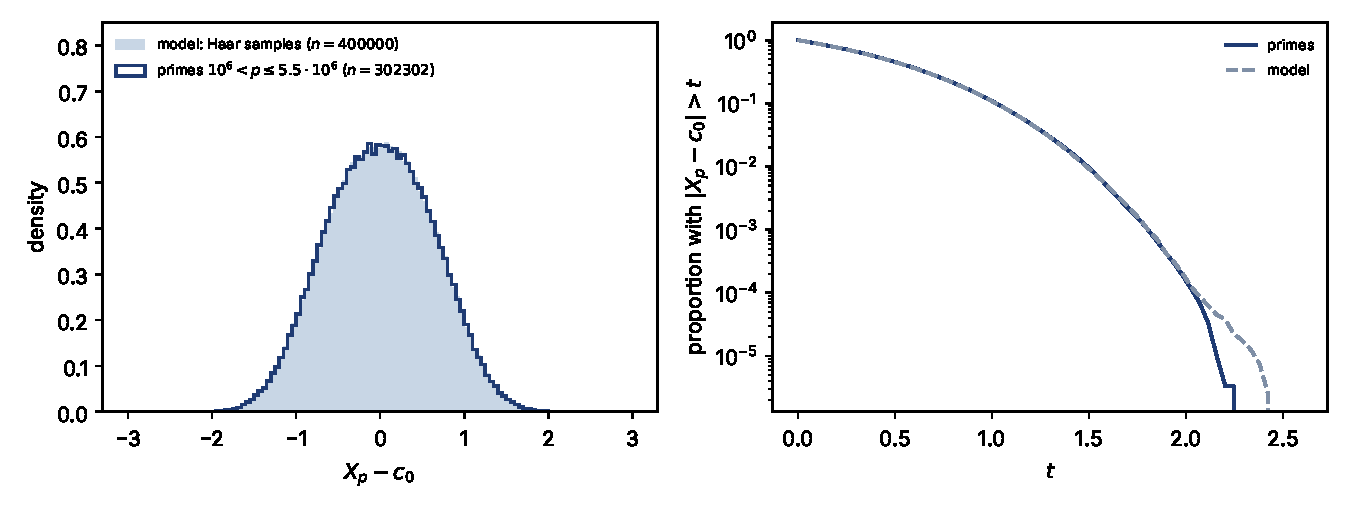
\includegraphics[width=\textwidth]{limit_law.pdf}
\caption{Left: the distribution of $X_p-c_0$ over the $302302$ primes in $(10^6,5.5\cdot10^6]$, against $4\cdot10^5$ Haar samples of $\frac4\pi R_{8001}$. Right: the proportion with $|X_p-c_0|>t$, on a log scale. The curves separate only near the sampling floor $1/n$.}
\label{fig:law}
\end{figure}

\begin{remark}[What is new here]
Part~(a) is the standard argument for limit-periodic functions in $B^2$: it uses Theorem~B(ii) and Lemma~9.3, with the Siegel--Walfisz theorem to pass to primes. The density statements in~(b) also follow, without~(a), from Theorems~E(ii) and~F and the Cauchy--Schwarz inequality, once one knows that
\[
\sup_q c_0(q;1)=+\infty\qquad\text{and}\qquad\inf_q c_0(q;-1)=-\infty .
\]
That is the computation \eqref{eq:condmean} at $Q=Q_K$, and it is the new input. In \cite{TS} the constants $c_0(q;r)$ appear only numerically \cite[Table~2]{TS}. We know of no earlier limiting-distribution result for $S(p)$. The limit laws of Vardi \cite{Vardi} for Dedekind sums and of Bettin and Drappeau \cite{BD} for cotangent sums average over all fractions $a/q$, whereas $S(p)$ involves one point per modulus.
\end{remark}


\section{The character expansion of the limit law}\label{sec:J}

The limit $R_\infty$ has an explicit expansion in Dirichlet characters. It gives exact formulas for $\sigma^2$ and for the constants $c_0(q;r)$ of Theorem~F, which \cite{TS} computed only numerically.

Let $\mathcal X$ be the set of odd primitive Dirichlet characters $\chi$ whose conductor $f=f_\chi$ is odd (so $f\ge3$). Every such $\chi$ defines a continuous character $x\mapsto\chi(x\bmod f)$ of $\Omega$. For $\chi\in\mathcal X$ let $\tau(\chi)$ be its Gauss sum, and put
\begin{gather*}
E(\chi)=\prod_{\ell\mid f}\Big(1-\frac1{\ell^2}\Big)^{-1}\prod_{\ell\nmid2f}\Big(1+\frac{(1-\chi(\ell))(1-\bar\chi(\ell)/\ell)}{(1-1/\ell)(\ell^2-1)}\Big),\\
W(\chi)=\frac{i\,\tau(\chi)\chi(2)}{4f\varphi(f)}\,(2-\bar\chi(2))^2\,L(1,\bar\chi)^2\,E(\chi),
\end{gather*}
the products running over primes $\ell$ and converging absolutely.

\begin{theorem}\label{thm:J}
\begin{enumerate}
\item[(a)] In $L^2(\Omega)$, $R_\infty=\sum_{\chi\in\mathcal X}W(\chi)\,\chi$.
\item[(b)] Consequently
\[
\sigma^2=\frac{16}{\pi^2}\sum_{\chi\in\mathcal X}|W(\chi)|^2=\frac1{\pi^2}\sum_{\chi\in\mathcal X}\frac{|2-\chi(2)|^4\,|L(1,\chi)|^4\,|E(\chi)|^2}{f\,\varphi(f)^2}.
\]
\item[(c)] For $q\ge1$ with odd part $q'$ and $(r,q)=1$, the constant of Theorem~F is the finite sum
\[
c_0(q;r)=c_0+\frac4\pi\sum_{\chi\in\mathcal X,\ f_\chi\mid q'}W(\chi)\chi(r).
\]
For example, $\mathcal X$ contains a single character of conductor $3$, namely $\chi_{-3}$, and
\[
c_0(3;\pm1)=c_0\pm\frac{\sqrt3\,\pi}{18}\cdot\frac98\prod_{\ell\equiv5\ (6)}\Big(1+\frac2{(\ell-1)^2}\Big)=c_0\pm0.398484\ldots,
\]
so $c_0(3;1)=0.638418\ldots$ and $c_0(3;2)=-0.158550\ldots$.
\end{enumerate}
\end{theorem}

The proof rests on two lemmas.

\begin{lemma}\label{lem:hT}
Let $\chi\in\mathcal X$ have conductor $f$. Then
\begin{gather*}
h(\chi):=\sum_{0<a<f/2}\chi(a)=\frac{\tau(\chi)}{\pi i}(2-\bar\chi(2))L(1,\bar\chi),\\
t(\chi):=\sum_{a\bmod f}\bar\chi(a)\tan\frac{\pi a}f=-\frac{2f}\pi(2\chi(2)-1)L(1,\bar\chi).
\end{gather*}
\end{lemma}

\begin{proof}
For $0<x<1$, $x\ne\frac12$, the square wave has the symmetrically convergent Fourier series $\mathbf 1_{(0,1/2)}(x)-\frac12=\sum_{n\ \mathrm{odd}}\frac{e(nx)}{\pi in}$. Put $x=a/f$, multiply by $\chi(a)$ and sum over $a$. Since $\sum_a\chi(a)=0$ and $\sum_a\chi(a)e(na/f)=\bar\chi(n)\tau(\chi)$ (because $\chi$ is primitive), we get $h(\chi)=\frac{\tau(\chi)}{\pi i}\sum_{n\ \mathrm{odd}}\frac{\bar\chi(n)}n$. As $\bar\chi$ is odd, this sum is $2\sum_{n>0\ \mathrm{odd}}\bar\chi(n)/n=(2-\bar\chi(2))L(1,\bar\chi)$.

For $t$, use $\pi\tan\pi x=-\sum_{n\in\Z}\frac1{x+\frac12+n}$ (summed symmetrically), so that $\pi\tan\frac{\pi a}f=-\sum_n\frac{2f}{2a+f(2n+1)}$. As $a$ runs modulo $f$ and $n$ over $\Z$, $k=2a+f(2n+1)$ runs once over the odd integers, with $a\equiv k\bar2\pmod f$, so $\bar\chi(a)=\chi(2)\bar\chi(k)$. Hence $t(\chi)=-\frac{2f}\pi\chi(2)\sum_{k\ \mathrm{odd}}\frac{\bar\chi(k)}k=-\frac{2f}\pi\chi(2)(2-\bar\chi(2))L(1,\bar\chi)$, which is the stated formula. (In both computations, the symmetric truncations of the double sum and of the sum over $k$ differ by $O(1/N)$.)
\end{proof}

\begin{lemma}\label{lem:Ghat}
Let $d\ge3$ be odd and let $\chi$ be a character modulo $d$. If $\chi$ is even, then $\sum_xG_d(x)\bar\chi(x)=0$. If $\chi$ is odd and induced by $\chi^*\in\mathcal X$ of conductor $f\mid d$, let $m'$ be the product of the primes dividing $d$ but not $f$. Then
\[
\frac1{\varphi(d)}\sum_{x\in(\Z/d\Z)^\times}G_d(x)\bar\chi(x)=\frac d{f\varphi(d)}\,h(\chi^*)\,t(\chi^*)\prod_{\ell\mid m'}(1-\chi^*(\ell))\Big(1-\frac{\bar\chi^*(\ell)}\ell\Big).
\]
\end{lemma}

\begin{proof}
$G_d$ is odd, which gives the first claim. For the second, substitute $u=jx$ in $\sum_x\bar\chi(x)\sum_{j}\tan(\pi jx/d)$. The left side becomes $\frac1{\varphi(d)}H\cdot T$, where
\[
H=\sum_{\substack{0<j<d/2\\(j,d)=1}}\chi^*(j),\qquad T=\sum_{u\in(\Z/d\Z)^\times}\bar\chi^*(u)\tan\frac{\pi u}d.
\] Remove the condition $(\cdot,m')=1$ by M\"obius inversion over $e\mid m'$.
\begin{itemize}
\item In $H$, the inner sums are $\chi^*(e)\sum_{0<i<d/(2e)}\chi^*(i)$. Since $d/e=f\cdot n$ with $n$ odd, the range $(0,fn/2)$ consists of $(n-1)/2$ full periods and one copy of $(0,f/2)$, so each inner sum is $\chi^*(e)h(\chi^*)$. This gives $H=h(\chi^*)\prod_{\ell\mid m'}(1-\chi^*(\ell))$.
\item In $T$, the inner sums are $\bar\chi^*(e)\sum_{u\bmod fn}\bar\chi^*(u)\tan(\pi u/(fn))$ with $n=d/(ef)$ odd. Writing $u=a+fb$ and using $\sum_{b<n}\tan(y+\pi b/n)=n\tan ny$ (proof of Lemma~9.2(a)), each is $\bar\chi^*(e)\,n\,t(\chi^*)$. This gives $T=\frac dft(\chi^*)\prod_{\ell\mid m'}(1-\bar\chi^*(\ell)/\ell)$.\qedhere
\end{itemize}
\end{proof}

Lemma~\ref{lem:hT} is classical (compare B.~C.~Berndt, \emph{Classical theorems on quadratic residues}, Enseign.\ Math.\ 22 (1976)). For the appearance of $|L(1,\chi)|^4$, compare Walum's formula for $\sum_hs(h,p)^2$ (H.~Walum, Illinois J.\ Math.\ 26 (1982)). We know of no earlier character expansion of a limit law for $S(p)$.

\begin{proof}[Proof of Theorem~\ref{thm:J}]
(a) Write $\widehat{G_d}(\chi^*)=\E[G_d\,\bar\chi^*]$. The continuous characters of the compact abelian group $\Omega$ are the functions $x\mapsto\chi(x\bmod f)$, for $\chi$ primitive of odd conductor $f$ (including the trivial character, $f=1$). They form an orthonormal basis of $L^2(\Omega)$. Fix $\chi^*$ of conductor $f$; the coefficient of $\chi^*$ in $G_d$ vanishes unless $f\mid d$, and is then given by Lemma~\ref{lem:Ghat}. It vanishes if $\chi^*$ is even (in particular if $f=1$). Since $|h(\chi^*)|\le f$, $|t(\chi^*)|\le\frac{2f}\pi\cdot3|L(1,\bar\chi^*)|$ and $d/\varphi(d)\ll\log\log d$, these coefficients are $\ll_{\chi^*}4^{\omega(d)}\log\log d$, so $\sum_d|\widehat{G_d}(\chi^*)|/d^2<\infty$. As $R_K\to R_\infty$ in $L^2$ and $w_d(K)\uparrow\pi^2/8$, dominated convergence gives
\[
\widehat{R_\infty}(\chi^*)=\frac{\pi^2}8\sum_{\substack{d\ \mathrm{odd}\\ f\mid d}}\frac{\widehat{G_d}(\chi^*)}{d^2}.
\]
Write $d=fm$ with $m$ odd. Then $\varphi(d)=\varphi(f)\,m\prod_{\ell\mid m'}(1-1/\ell)$, and Lemma~\ref{lem:Ghat} turns the sum into $\frac{h(\chi^*)t(\chi^*)}{f^2\varphi(f)}\sum_{m\ \mathrm{odd}}m^{-2}g(m)$. Here $g$ is multiplicative, $g(\ell^v)=1$ for $\ell\mid f$, and $g(\ell^v)=\frac{(1-\chi^*(\ell))(1-\bar\chi^*(\ell)/\ell)}{1-1/\ell}$ for $\ell\nmid f$. The Euler product of $\sum_mg(m)m^{-2}$ is $E(\chi^*)$. Finally, Lemma~\ref{lem:hT} gives $h(\chi^*)t(\chi^*)=-\frac{2f\tau(\chi^*)\chi^*(2)}{\pi^2i}(2-\bar\chi^*(2))^2L(1,\bar\chi^*)^2$, using $2\chi(2)-1=\chi(2)(2-\bar\chi(2))$. So $\widehat{R_\infty}(\chi^*)=W(\chi^*)$.

(b) Parseval's identity, with $|\tau(\chi)|^2=f$ and $|2-\bar\chi(2)|=|2-\chi(2)|$.

(c) By Theorem~\ref{thm:G}(c), $c_0(q;r)-c_0$ is $\frac4\pi$ times the conditional mean of $R_\infty$ given $x\equiv r\pmod{q'}$. That conditional expectation is the orthogonal projection onto the span of the characters that factor through $(\Z/q'\Z)^\times$, i.e.\ those with $f_\chi\mid q'$. For $q=3$: $\tau(\chi_{-3})=i\sqrt3$, $\chi_{-3}(2)=-1$, $L(1,\chi_{-3})=\pi/(3\sqrt3)$, and $E(\chi_{-3})=\frac98\prod_{\ell\equiv5\,(6)}(1+2/(\ell-1)^2)=1.318174\ldots$.
\end{proof}

\begin{remark}[Numerical checks]\label{rem:Jnum}
\begin{itemize}
\item Lemmas~\ref{lem:hT} and~\ref{lem:Ghat} agree with direct evaluation of $h$, $t$ and the Fourier coefficients of $G_d$ to $10^{-12}$ (all odd characters modulo $d=9$, $15$, $21$, $25$, $27$, $35$, $45$, $63$).
\item Formula~(c) reproduces every entry of Table~2 of~\cite{TS} for $q=3,5,7,9$ to the four digits printed, except $c_0(9;8)=-0.28905$, which Table~2 of~\cite{TS} rounds to $-0.2891$ (within its stated uncertainty). For instance, it gives $c_0(5;1)=0.5863$, $c_0(5;2)=0.4159$, $c_0(7;1)=0.4656$ and $c_0(9;1)=0.7689$. \cite{TS} obtained these by summing over $d\le8001$ and extrapolating.
\item Beyond Table~2, formula~(c) was tested against the primes themselves. For every odd $q\le45$ and every $r$ ($422$ classes, with predicted values from $-0.621$ to $1.101$), the mean of $X_p$ over the primes $10^3<p\le5.5\cdot10^6$ in the class agrees with $c_0(q;r)$ to within $1.4$ standard errors, and to within $0.0072$ in absolute terms (\texttt{data/class\_means\_theoremJ\_q45.txt}).
\item The series in~(b), summed over the conductors $f\le F$, gives $0.389678$, $0.391018$, $0.391467$, $0.391692$, $0.391827$, $0.392008$ and $0.392098$ for $F=401,801,1201,1601,2001,3001,4001$. Its tail is $\approx a/F$, and extrapolation gives $\sigma^2=0.392369\pm0.000002$ ($\sigma=0.626393$; the spread is over fits of the tail by $a/F$, $a/F+b/F^2$ and $(a+b\log F)/F$), in agreement with the value $0.3924\pm0.0001$ found above by a different method.
\end{itemize}
The code is \texttt{code/char\_expansion.py}.
\end{remark}


\begin{corollary}[Classes with smooth moduli]\label{cor:smoothclass}
Let $Q_K=\prod_{3\le\ell<K}\ell^{a_\ell}$, with $a_\ell$ minimal such that $\ell^{a_\ell}>K^3$. As $K\to\infty$,
\[
c_0(Q_K;\pm1)=c_0\pm\Big(\kappa_H\log K\,\big(\log K-\gamma-\log2+K_0\big)+C_Q+o(1)\Big),\qquad\kappa_H=\frac{2e^\gamma}{\pi^2},
\]
where $C_Q=-\frac4\pi\sum_{e\ \mathrm{odd}}\frac1e\Big(\frac{\log e+K_0}\pi-\frac{F_e(1)}e\Big)=-0.35153\ldots$ (the term $e=1$ has $F_1(1)=0$).
\end{corollary}

\begin{proof}
By (9.2) and the proof of Theorem~\ref{thm:G}(b), $c_0(Q;\pm1)-c_0=\pm\frac\pi2\sum_{d\mid Q,\,d\ge3}G_d(1)/d^2+o(1)$ for $Q=Q_K$. Möbius inversion of Lemma~9.1 gives $G_d=\sum_{e\mid d}\mu(d/e)F_e$ (with $F_1=0$), hence
\[
\sum_{d\mid Q}\frac{G_d(1)}{d^2}=\sum_{e\mid Q}\frac{F_e(1)}{e^2}\prod_{\ell\mid Q/e}\Big(1-\frac1{\ell^2}\Big).
\]
The product equals $\prod_{3\le\ell<K}(1-\ell^{-2})=\frac8{\pi^2}(1+O(K^{-1}))$, unless $\ell^{a_\ell}\mid e$ for some $\ell$. The $e$ of that exceptional kind contribute $O((\log K)^2K^{-2})$, since $\ell^{-a_\ell}<K^{-3}$. By Corollary~4.3(a), $F_e(1)/e^2=(\log e+K_0)/(\pi e)+O(e^{-3})$. Truncating at the exponents $a_\ell$ changes the Euler products below by factors $1+O(K^{-2})$. So
\[
\sum_{e\mid Q}\frac{\log e+K_0}e=E_K\Big(\sum_{3\le\ell<K}\frac{\log\ell}{\ell-1}+K_0\Big)(1+O(K^{-2})),\qquad E_K=\prod_{3\le\ell<K}\Big(1-\frac1\ell\Big)^{-1}.
\]
By the prime number theorem with error term, $E_K=\frac{e^\gamma}2\log K\,(1+O(e^{-c\sqrt{\log K}}))$ and $\sum_{3\le\ell<K}\frac{\log\ell}{\ell-1}=\log K-\gamma-\log2+O(e^{-c\sqrt{\log K}})$. Collecting, $\frac\pi2\sum_{d\mid Q}G_d(1)/d^2=\frac\pi2\cdot\frac8{\pi^2}\cdot\frac{e^\gamma}{2\pi}\log K(\log K-\gamma-\log2+K_0)+O(1)$, up to the $O(1)$ terms. These are the term $e=1$ and the remainders of Corollary~4.3(a), which together sum to $C_Q$; every other error is $o(1)$.
\end{proof}

\begin{remark}
Exact values of $\frac\pi2\sum_{d\mid Q_K}G_d(1)/d^2$ are $15.89$, $28.84$ and $45.64$ for $K=10^3,10^4,10^5$. The two-term formula gives $16.10$, $29.12$ and $45.96$: the differences $-0.21,-0.28,-0.32$ approach $C_Q=-0.3515$; the remaining drift comes from the Mertens-product error at these $K$. The leading term $\kappa_H(\log K)^2$ alone is off by $1.3$, $1.8$ and $2.2$. Note $-\gamma-\log2+K_0=-0.4515\ldots$.
\end{remark}

\section{Extreme values}\label{sec:H}

Here we prove the extreme-value theorem, with the same constant as the tails below. The proof transfers the deterministic contribution of the small moduli, computed in Lemma~\ref{lem:det}, to the primes of one residue class, using Gallagher's prime number theorem. For that, only an upper bound for a mean square and a lower bound for the size of the class are needed.

\begin{theorem}\label{thm:H}
For every $\varepsilon>0$ there is $X_0(\varepsilon)$ such that for $X\ge X_0(\varepsilon)$ there are primes $p,p'\in(X,2X]$ with
\[
X_p\le c_0-(\kappa_H-\varepsilon)(\log\log p)^2,\qquad X_{p'}\ge c_0+(\kappa_H-\varepsilon)(\log\log p')^2,\qquad\kappa_H=\frac{2e^\gamma}{\pi^2}.
\]
In fact each inequality holds for at least $X^{1-o(1)}$ primes in $(X,2X]$. The constant $X_0(\varepsilon)$ is effectively computable.
\end{theorem}

Thus $X_p-c_0=\Omega_\pm((\log\log p)^2)$ unconditionally and effectively. Together with \cite[Theorem~E]{TS}, which gives $X_p-c_0=O((\log\log p)^2)$ for all $p$ outside a set of density zero, this shows that $(\log\log p)^2$ is the true order of the extreme deviations.

\subsection{External input}

We use the following two results, for Dirichlet characters to moduli $r\le R$. A real zero $\tilde\beta$ of $L(s,\tilde\chi)$, with $\tilde\chi$ primitive of conductor $\tilde q\le R$, is \emph{exceptional of level $R$ and quality $\delta$} if $\tilde\beta\ge1-\delta/\log R$.

\begin{enumerate}
\item[(LP)] (Landau--Page.) There is an absolute $\delta_0\in(0,1)$ such that for all large $R$ there is at most one exceptional zero of level $R$ and quality $\delta_0$. If it exists, $\tilde\chi$ is real and $\tilde\beta$ is simple.
\item[(Ga)] (Gallagher, \emph{Invent.\ Math.}\ 11 (1970), 329--339, Theorem~7.) There are absolute constants $b_G,c>0$ such that the following holds for $\exp((\log N)^{1/2})\le R\le N^{b_G}$ and $0<\delta<1$:
\[
\sum_{r\le R}\ \sideset{}{^*}\sum_{\chi\bmod r}\ \max_{I\subset[1,N]}\frac1{|I|+N/R}\Big|\sum_{n\in I}\big(\Lambda(n)\chi(n)-\mathbf 1_{r=1}+\mathbf 1_{\chi=\tilde\chi}\,n^{\tilde\beta-1}\big)\Big|\ll E_\delta(N,R).
\]
Here $E_\delta=\exp(-c\delta\log N/\log R)$ if there is no exceptional zero of level $R$ and quality $\delta$, and then the term with $\tilde\chi$ is omitted. Otherwise $E_\delta=\exp(-c\log N/\log R)$. (We use the formulation of Lemma~7.3 of L.~Grimmelt and J.~Ter\"av\"ainen, arXiv:2508.16400, but only in Gallagher's range $R\le N^{b_G}$. The range $R\le N$ stated there is too generous near $R=N$; their paper uses only $R\le N^{1/7}$.)
\end{enumerate}

With $\delta=\delta_0$, both cases give $E_{\delta_0}\ll\exp(-c_2\log N/\log R)$ with $c_2=c\delta_0$.

\subsection{Primes in a class, tested against periodic functions}

For odd $Q$ and $(a,Q)=1$ write $\E[\,\cdot\mid a]=\E[\,\cdot\mid x\equiv a\pmod Q]$ on $\Omega$. Let $\mathcal P=\mathcal P_X(a,Q)$ be the set of primes $p\in(X,2X]$ with $p\equiv a\pmod Q$.

\begin{lemma}\label{lem:Ga}
Let $X$ be large and $\exp(\sqrt{\log 2X})\le T\le X^{b_G}$, where we may assume $b_G\le\frac14$. Let $Q$ be odd with $(a,Q)=1$, and let $f$ be a function on the reduced residues modulo an odd $M$ with $\mathrm{lcm}(M,Q)\le T$. Then
\[
\sum_{p\in\mathcal P}f(p)\log p=\frac X{\varphi(Q)}\Big(\E[f\mid a]-\theta\,\E[f\tilde\chi\mid a]\Big)+O\Big(\frac{\|f\|_\infty X}{\varphi(Q)}e^{-c_2\log X/\log T}\Big).
\]
If there is an exceptional zero $\tilde\beta$ of level $T$ and quality $\delta_0$, then $\tilde\chi$ is its character and $\theta=X^{-1}\sum_{X<n\le2X}n^{\tilde\beta-1}\in(0,1]$; otherwise $\theta=0$. The number $\theta$ depends only on $X$ and $T$.
\end{lemma}

\begin{proof}
Put $M'=\mathrm{lcm}(M,Q)$ and $I=(X,2X]$. Expanding $f\cdot\mathbf 1_{x\equiv a(Q)}$ in characters modulo $M'$,
\[
\sum_{\substack{n\in I\\ n\equiv a(Q)}}\Lambda(n)f(n)=\sum_{\chi\bmod M'}\hat f(\chi)\sum_{n\in I}\Lambda(n)\chi(n),\qquad\hat f(\chi)=\frac1{\varphi(M')}\sum_{\substack{x\bmod M'\\ x\equiv a(Q)}}f(x)\bar\chi(x).
\]
The inner sum has $\varphi(M')/\varphi(Q)$ terms, so $|\hat f(\chi)|\le\|f\|_\infty/\varphi(Q)$.

Each $\chi\bmod M'$ is induced by a unique primitive $\chi^*$ of conductor $r\mid M'$, $r\le T$, and the two sums over $n\in I$ differ by $O(\log M'\log X)$. By (Ga) with $N=2X$, $R=T$ (so $|I|+N/R\le3X$), and by $\sum_{n\in I}n^{\tilde\beta-1}=\theta X$:
\begin{itemize}
\item the principal character contributes $\hat f(\chi_0)X=\frac X{\varphi(Q)}\E[f\mid a]$;
\item the character induced by $\tilde\chi$, present only when $\tilde q\mid M'$, contributes $-\hat f(\tilde\chi)\theta X=-\frac{\theta X}{\varphi(Q)}\E[f\tilde\chi\mid a]$;
\item all characters together contribute an error $O(\|f\|_\infty\varphi(Q)^{-1}(Xe^{-c_2\log X/\log T}+T\log^2X))$.
\end{itemize}
If $\tilde q\nmid M'$, we set $\E[f\tilde\chi\mid a]=0$. This is consistent: when $\tilde q$ is odd, the expectation computed modulo $\mathrm{lcm}(M',\tilde q)$ vanishes; indeed, $\tilde q$ is then squarefree, so some prime $\ell\mid\tilde q$ does not divide $M'$. (When $4\mid\tilde q$ the character never occurs in the expansion modulo the odd number $M'$.) The corresponding local component of $x$ is uniform and independent of $x\bmod M'$ on $\{x\equiv a\ (Q)\}$, and the local component of $\tilde\chi$ is nontrivial. So the formula holds in all cases.

Prime powers contribute $O(\|f\|_\infty X^{1/2}\log X)$, and $T\log^2X+X^{1/2}\log X\ll Xe^{-c_2\log X/\log T}/\varphi(Q)$ since $\varphi(Q)\le T\le X^{1/4}$ and $e^{-c_2\log X/\log T}\ge e^{-c_2\sqrt{\log X}}$.
\end{proof}

\subsection{The random part is small in mean square}

Fix $K\ge5$, $Q=Q_K=\prod_{3\le\ell<K}\ell^{a_\ell}$ (with $a_\ell$ minimal such that $\ell^{a_\ell}>K^3$), any $a$ coprime to $Q$, and $Y>Q$. Put
\[
R'_a(x)=\sum_{\substack{3\le d<Y\\ d\nmid Q}}\frac{w_d(Y)}{d^2}G_d(x).
\]

\begin{lemma}\label{lem:R'}
$\E[R_a'^2\mid a]\le\eta(K)$, where $\eta(K)\to0$ as $K\to\infty$ uniformly in $Y$ and $a$.
\end{lemma}

\begin{proof}
Under $\Prob(\,\cdot\mid a)$ the components of $x$ at the various primes are independent. At $\ell<K$ the residue $x\bmod\ell^{a_\ell}$ is fixed and the higher $\ell$-adic digits are uniform; at $\ell\ge K$ the unit $x\in\Z_\ell^\times$ is Haar distributed.

For $d$ let $\mathcal S(d)$ be the set of primes $\ell\mid d$ at which $x\bmod\ell^{v_\ell(d)}$ is not determined by the condition. These are the $\ell\ge K$, and the $\ell<K$ with $v_\ell(d)>a_\ell$. Then $d\nmid Q$ if and only if $\mathcal S(d)\ne\emptyset$. For a pair $d,d'$ put $\mathcal S_0=\mathcal S(d)\cap\mathcal S(d')$, and let $\xi$ be the $\mathcal S_0$-components of $x$.

Conditionally on $\xi$, the values $G_d(x)$ and $G_{d'}(x)$ depend on disjoint sets of independent components. So
\[
\E[G_dG_{d'}\mid a]=\E_\xi\big[\E[G_d\mid a,\xi]\,\E[G_{d'}\mid a,\xi]\big],
\]
and this equals $\E[G_d\mid a]\E[G_{d'}\mid a]$ if $\mathcal S_0=\emptyset$. Moreover $\E[G_d\mid a,\xi]=A^*_{d,g}(s)$ for some $s$, where $g=g_d\mid d$ is the part of $d$ at which $x$ is determined by $a$ and $\xi$; explicitly $g_d=(d_0,Q)\,d_1$ in the notation below. By Lemma~9.2(c) (and $A^*_{d,1}=0$) this has absolute value at most $C\tau(d)^2\lambda(d)\,g_d$.

Write $c_d=w_d(Y)/d^2\le\frac{\pi^2}8d^{-2}$. Then
\[
\E[R_a'^2\mid a]\le\Big(\sum_{d\nmid Q}|c_d|\,|\E[G_d\mid a]|\Big)^2+C^2\!\!\sum_{\mathcal S_0\neq\emptyset}|c_dc_{d'}|\,\tau(d)^2\tau(d')^2\lambda(d)\lambda(d')\,g_dg_{d'} .
\]

\emph{The first term.} $\E[G_d\mid a]=A^*_{d,(d,Q)}(a)$, so the first term tends to $0$ by the three-case estimate in the proof of Theorem~\ref{thm:G}(b). That estimate uses only Lemma~9.2(c), so it is uniform in $a$.

\emph{The second term.} For a pair with $\mathcal S_0\ne\emptyset$, write $d=d_0d_1$, where $d_1=\prod_{\ell\in\mathcal S_0}\ell^{v_\ell(d)}$ is the full $\mathcal S_0$-part of $d$. Then $g_d\le(d_0,Q)\,d_1$. Use $\tau(mn)\le\tau(m)\tau(n)$, $\lambda(mn)\le\lambda'(m)\lambda'(n)$ and $\lambda'(mn)\le2\lambda'(m)\lambda'(n)$, and write $d_0=(d_0,Q)\,u$. Then the contribution of $d$ is at most
\[
\frac{\tau(d)^2\lambda(d)\,g_d}{d^2}\le\frac{\tau((d_0,Q))^2\lambda'((d_0,Q))}{(d_0,Q)}\cdot\frac{\tau(u)^2\lambda'(u)}{u^2}\cdot\frac{\tau(d_1)^2\lambda'(d_1)}{d_1}.
\]
For $\ell\in\mathcal S_0$ we have $v_\ell(d)\ge1$ if $\ell\ge K$, and $v_\ell(d)\ge a_\ell+1$ if $\ell<K$. Summing over all pairs, the second term is at most
\[
C\Big(\sum_{g\mid Q}\frac{\tau(g)^2\lambda'(g)}g\Big)^2\Big(\sum_{u\ge1}\frac{\tau(u)^2\lambda'(u)}{u^2}\Big)^2\sum_{\mathcal S_0\neq\emptyset}\ \prod_{\ell\in\mathcal S_0}\Big(2\sum_{v\ge m_\ell}\frac{(v+1)^2\lambda'(\ell^v)}{\ell^v}\Big)^2,
\]
with $m_\ell=1$ for $\ell\ge K$ and $m_\ell=a_\ell+1$ for $\ell<K$.
\begin{itemize}
\item The first factor is $(\log K)^{O(1)}$ (as in the proof of Theorem~\ref{thm:G}(b), first bullet, using $\lambda'(g)\ll(\log K)^3g^{1/\log K}$).
\item The second factor is $O(1)$.
\item Each local factor is $\ll(\log\ell)^3/\ell^2$ for $\ell\ge K$, and $\ll(\log K)^{O(1)}K^{-6}$ for $\ell<K$ (since $\ell^{a_\ell}>K^3$). So the last sum is at most $\exp\big(C\sum_{\ell\ge K}(\log\ell)^3\ell^{-2}+(\log K)^{O(1)}K^{-5}\big)-1\ll(\log K)^3K^{-1}$.
\end{itemize}
Hence the second term is $\ll(\log K)^{O(1)}K^{-1}\to0$.
\end{proof}

\subsection{The deterministic part}

\begin{lemma}\label{lem:det}
Let $\epsilon\in\{1,-1\}$, $Q=Q_K$, and $a\equiv\epsilon\pmod Q$. Put $D(a)=\sum_{d\mid Q,\,d\ge3}w_d(Y)G_d(a)/d^2$ with $Y>Q$. Then $\epsilon D(a)\ge(\frac{e^\gamma}{2\pi}-o(1))(\log K)^2$ as $K\to\infty$.
\end{lemma}

\begin{proof}
Since $a\equiv\epsilon\pmod d$ for all $d\mid Q$, we have $\epsilon D(a)=\sum_{d\mid Q}w_d(Y)G_d(1)/d^2$, and every $G_d(1)$ is positive. For $m\mid Q/d$ we have $dm\le Q<Y$, so $w_d(Y)\ge\sum_{m\mid Q/d}m^{-2}$. By Lemma~9.1 (the divisors of $Q$ are closed under taking divisors) and Corollary~4.3(a), this is at least
\[
\sum_{k\mid Q,\,k\ge3}\frac{F_k(1)}{k^2}\ge\frac1\pi\sum_{k\mid Q}\frac{\log k}k-1 .
\]
Next,
\[
\sum_{k\mid Q}\frac{\log k}k\ \ge\ \sum_{3\le\ell<K}\log\ell\sum_{\substack{k\mid Q\\ \ell\mid k}}\frac1k\ \ge\ \sum_{3\le\ell<K}\frac{\log\ell}{\ell}\Big(1-\frac1\ell\Big)\prod_{3\le\ell'<K}\sum_{b\le a_{\ell'}}\ell'^{-b}.
\]
The product is at least $(1-K^{-2})\prod_{3\le\ell'<K}(1-1/\ell')^{-1}=(\frac{e^\gamma}2+o(1))\log K$ by Mertens. So $\epsilon D(a)\ge(\frac{e^\gamma}{2\pi}+o(1))(\log K)^2$.
\end{proof}

\subsection{Proof of Theorem~\ref{thm:H}}\label{sec:Hproof}

Let $c_2$ be as after (Ga), let $X$ be large, and put
\[
\log T_0=\frac{c_2\log X}{20\log\log X}.
\]
Let $K$ be maximal such that $Q:=Q_K$ satisfies $Q^3(\log X)^{32}\le T_0$, and put
\[
Y=Q(\log X)^{16},\qquad T=QY^2\le T_0 .
\]
Since $\log Q_K=(4+o(1))K$, we get $K=(\frac{c_2}{240}+o(1))\log X/\log\log X$, hence $\log K=(1+o(1))\log\log X$. Also $T\ge\exp(\sqrt{\log X})$ and $Q=X^{o(1)}$.

\emph{Choice of the class.} Fix $\epsilon=-1$ for $p$, or $\epsilon=+1$ for $p'$.
\begin{itemize}
\item If there is no exceptional zero of level $T$ and quality $\delta_0$, or if its conductor $\tilde q$ does not divide $Q$, take $a\equiv\epsilon\pmod Q$.
\item Otherwise $\tilde q\mid Q$. This exceptional case is treated in Section~\ref{sec:exc}.
\end{itemize}
In the first case, Lemma~\ref{lem:det} gives
\[
\epsilon D(a)\ge\Big(\frac{e^\gamma}{2\pi}-o(1)\Big)(\log K)^2 .
\]

\emph{Decomposition.} Let $p\in\mathcal P=\mathcal P_X(a,Q)$ and $K_2=\sqrt{2X}(\log2X)^4$. By Theorem~B(ii) and Lemma~9.1,
\[
X_p-c_0=\frac4\pi\Big(D(a)+R'_a(p)+V(p)\Big)+O\Big(\frac1{\log X}\Big),\qquad V=R_{K_2}-R_Y ,
\]
because $G_d(p)=G_d(a)$ for $d\mid Q$.

\emph{Size of the class.} By Lemma~\ref{lem:Ga} with $f\equiv1$ and $M=1$,
\[
\sum_{p\in\mathcal P}\log p=\frac X{\varphi(Q)}+O\Big(\frac X{\varphi(Q)}(\log X)^{-20}\Big)\ge(1-o(1))\frac X{\varphi(Q)},
\]
since $c_2\log X/\log T\ge20\log\log X$ (as $\tilde q\nmid Q$, there is no exceptional term).

\emph{Second moment of $R'_a$.} Apply Lemma~\ref{lem:Ga} to each $f=G_dG_{d'}$ ($d,d'<Y$, $d,d'\nmid Q$, $M=\mathrm{lcm}(d,d')$, $\mathrm{lcm}(M,Q)\le T$), multiply by $c_dc_{d'}$ and sum. The main terms add up to $\frac X{\varphi(Q)}\E[R_a'^2(1-\theta\tilde\chi)\mid a]\le\frac{2X}{\varphi(Q)}\E[R_a'^2\mid a]$, because $R_a'^2\ge0$ and $0\le\theta\le1$. By Lemma~9.2(b), $\sum_{d<Y}|c_d|\,\|G_d\|_\infty\ll(\log Y)^3$, so the errors add up to $O(X\varphi(Q)^{-1}(\log Y)^6(\log X)^{-20})$. With Lemma~\ref{lem:R'}:
\[
\sum_{p\in\mathcal P}R'_a(p)^2\log p\le\frac{2X}{\varphi(Q)}\eta(K)+o\Big(\frac X{\varphi(Q)}\Big)=o\Big(\frac X{\varphi(Q)}\Big).
\]

\emph{The tail $V$.} By Lemmas~9.3(b) and~9.4 over all integers,
\[
\sum_{p\in\mathcal P}V(p)^2\log p\le\log(2X)\sum_{X<n\le2X}V(n)^2\ll\frac{X(\log X)^{15}}Y=\frac X{Q\log X}=o\Big(\frac X{\varphi(Q)}\Big).
\]

\emph{Conclusion.} The $\log$-weighted proportion of $p\in\mathcal P$ with $|R'_a(p)+V(p)|>1$ is $o(1)$. For all other $p\in\mathcal P$,
\[
\epsilon(X_p-c_0)\ge\frac4\pi\Big(\frac{e^\gamma}{2\pi}-o(1)\Big)(\log K)^2-O(1)=(\kappa_H-o(1))(\log\log p)^2 .
\]
Such primes number at least $(1-o(1))X/(\varphi(Q)\log X)=X^{1-o(1)}$. This proves Theorem~\ref{thm:H} unless $\tilde q\mid Q$; that case is treated in Section~\ref{sec:exc}.

\begin{remark}
\emph{Context.} The method is a transfer of standard tools: Gallagher's prime number theorem at moduli $\exp(c\log X/\log\log X)$, a mean-square bound so that only an upper bound is needed, and, for the exceptional character, the removal of one prime from $Q$ (Section~\ref{sec:exc}), which replaces Siegel's theorem. An analogous unconditional result for $L(1,\chi)$ is due to Joshi (P.~T.~Joshi, \emph{J. Number Theory} 2 (1970), 58--73): $L(1,(\cdot/q))\ge(e^\gamma-\varepsilon)\log\log q$ for infinitely many primes $q$.

\emph{Why GRH is not needed.} An asymptotic for each class separately would need GRH. Here only an \emph{upper} bound for a nonnegative quantity is needed, together with a lower bound for the size of one class. Gallagher's theorem gives both with relative error $\exp(-c\log X/\log T)$, which is a negative power of $\log X$ once $\log T\asymp\log X/\log\log X$. This modulus is still large enough that $\log K\sim\log\log X$.
\end{remark}

\subsection{The exceptional case}\label{sec:exc}

It remains to treat the case where there is an exceptional zero $\tilde\beta$ of level $T$ and quality $\delta_0$ whose conductor $\tilde q$ divides $Q$. The usual tool here is Siegel's theorem, which is ineffective. Instead we remove one prime from $Q$.



\begin{proof}[Proof of Theorem~\ref{thm:H} in the exceptional case]
Let $\ell_1$ be the largest prime factor of $\tilde q$, which is odd and squarefree.

\emph{$\ell_1$ is large, effectively.} For a real primitive character of conductor $\tilde q$, every real zero satisfies $1-\tilde\beta\ge c_P\,\tilde q^{-1/2}(\log\tilde q)^{-2}$, with $c_P>0$ effective \cite[Chapter~14]{Dav}. With $1-\tilde\beta\le\delta_0/\log T$ this gives $\log\tilde q\ge(2-o(1))\log\log T$. Also $\tilde q\le\prod_{\ell\le\ell_1}\ell\le e^{1.02\ell_1}$ and $\log\log T=(1+o(1))\log K$, so $\ell_1\ge(1.9+o(1))\log K$; in particular $\ell_1\to\infty$ (only this is needed below).

\emph{The class.} Put $Q'=Q/\ell_1^{a_{\ell_1}}$ and take $a\equiv\epsilon\pmod{Q'}$. Since $\ell_1\nmid Q'$, $\tilde q\nmid Q'$. Let $\mathcal P'=\mathcal P_X(a,Q')$. By Lemma~\ref{lem:Ga} with $f\equiv1$ and $M=1$, there is no exceptional term, and $\sum_{p\in\mathcal P'}\log p=(1+o(1))X/\varphi(Q')$.

\emph{Decomposition.} With $c_d=w_d(Y)/d^2$, for $p\in\mathcal P'$,
\[
R_Y(p)=D'(a)+U(p)+R''(p),\qquad D'(a)=\sum_{d\mid Q',\,d\ge3}c_dG_d(a),\quad U=\sum_{\substack{d\mid Q\\ \ell_1\mid d}}c_dG_d,\quad R''=\sum_{\substack{3\le d<Y\\ d\nmid Q}}c_dG_d .
\]
\begin{itemize}
\item \emph{$D'$.} Every $d\mid Q'$ satisfies $a\equiv\epsilon\pmod d$, so $G_d(a)=\epsilon G_d(1)$. The argument for the first sum in the proof of Lemma~\ref{lem:det}, applied to $Q'$ in place of $Q$, gives $\epsilon D'(a)\ge\frac1\pi\sum_{k\mid Q'}\frac{\log k}k-1$. Compared with $Q$, the Mertens product loses the factor $1-1/\ell_1$, and the sum over $\ell$ loses the term $\ell=\ell_1$, which is at most $\frac{\log\ell_1}{\ell_1}$. Since $\ell_1\to\infty$, $\epsilon D'(a)\ge(\frac{e^\gamma}{2\pi}-o(1))(\log K)^2$.
\item \emph{$U$, pointwise.} By Lemma~\ref{lem:Gmax} below, $G_d(1)\le F_d(1)$ (Lemma~9.1, positivity) and Corollary~4.3(b),
\[
|U|\le\frac{\pi^2}8\sum_{\substack{d\mid Q\\ \ell_1\mid d}}\frac{\log d+K_0}{\pi d}\ll\frac1{\ell_1}\sum_{g\mid Q'}\frac{\log g+\log\ell_1+1}g\ll\frac{(\log K)^2}{\ell_1}=o\big((\log K)^2\big).
\]
\item \emph{$R''$, in mean square.} Apply Lemma~\ref{lem:Ga} with $Q'$ in place of $Q$ to $f=G_dG_{d'}$ ($d,d'<Y$, $d,d'\nmid Q$). As in Section~\ref{sec:Hproof}, the main terms add up to $\frac X{\varphi(Q')}\E[R''^2(1-\theta\tilde\chi)\mid a]\le\frac{2X}{\varphi(Q')}\E[R''^2\mid a]$, where now the condition is $x\equiv a\pmod{Q'}$. Conditioning further on $x\bmod\ell_1^{a_{\ell_1}}$ fixes $x\bmod Q$, and $R''$ is the function $R'_{a'}$ of Lemma~\ref{lem:R'} for the resulting class $a'\bmod Q$. Since that lemma is uniform in $a'$, $\E[R''^2\mid a]\le\eta(K)$. The error terms are as before.
\item \emph{The tail $V=R_{K_2}-R_Y$} is unchanged.
\end{itemize}
As in Section~\ref{sec:Hproof}, all but a $\log$-weighted proportion $o(1)$ of $p\in\mathcal P'$ satisfy $|R''(p)+V(p)|\le1$. For them,
\[
\epsilon(X_p-c_0)\ge\frac4\pi\Big(\epsilon D'(a)-|U(p)|-1\Big)+O\Big(\frac1{\log X}\Big)\ge(\kappa_H-o(1))(\log\log p)^2,
\]
and there are $X^{1-o(1)}$ of them. Every $o(1)$ here is effective.
\end{proof}

\begin{remark}[Effectivity]
All the inputs are effective: (LP); Gallagher's theorem (Ga), whose constants $b_G,c$ are effective because his proof uses only the log-free zero-density estimate and the Deuring--Heilbronn phenomenon; the prime number theorem (for $\log Q_K$) and Mertens' theorems; Theorem~B(ii); and Lemmas~9.2--9.4, \ref{lem:R'} and~\ref{lem:det}, whose constants are explicit. Hence the constant $X_0(\varepsilon)$ in Theorem~\ref{thm:H} is effectively computable.
\end{remark}


\section{Tails, moments, and a conjecture}\label{sec:I}

\subsection{Tails of the limiting distribution}

Lemmas~\ref{lem:R'} and~\ref{lem:det} also describe the tails of the law $\nu$ of Theorem~\ref{thm:G}.

\begin{corollary}\label{cor:tails}
As $t\to\infty$,
\[
\nu\big((-\infty,c_0-t)\big)\ \ge\ \exp\Big(-\exp\big((1+o(1))\sqrt{t/\kappa_H}\big)\Big),
\]
and the same lower bound holds for $\nu\big((c_0+t,\infty)\big)$. Consequently, as $t\to\infty$, the primes with $S(p)<\frac p2\log p+(c_0-t)p$, and also the primes with $S(p)>\frac p2\log p+(c_0+t)p$, have lower density at least $\exp(-\exp((1+o(1))\sqrt{t/\kappa_H}))$.
\end{corollary}

\begin{proof}
Let $\epsilon=\mp1$, and let $\mathcal C=\{x\equiv\epsilon\pmod{Q_K}\}$, so that $\Prob(\mathcal C)=1/\varphi(Q_K)\ge e^{-(4+o(1))K}$. On $\mathcal C$ we have
\[
R_\infty=D_\infty+R'_\infty,\qquad D_\infty=\frac{\pi^2}8\sum_{d\mid Q_K,\,d\ge3}\frac{G_d(\epsilon)}{d^2}.
\]
Here $R'_\infty$ is the $L^2$ limit, as $Y\to\infty$, of $R'_a$ in Lemma~\ref{lem:R'} with $a=\epsilon$; it exists by Lemma~\ref{lem:L2}.
\begin{itemize}
\item By Lemma~\ref{lem:R'}, $\E[R_\infty'^2\mid\mathcal C]\le\eta(K)\to0$, so $\Prob(|R'_\infty|\le1\mid\mathcal C)\ge\frac12$ for large $K$.
\item By Lemma~\ref{lem:det}, and $w_d\to\pi^2/8$, we have $\epsilon D_\infty\ge(\frac{e^\gamma}{2\pi}-o(1))(\log K)^2$.
\end{itemize}
Hence $\epsilon\cdot\frac4\pi R_\infty\ge(\kappa_H-o(1))(\log K)^2-\frac4\pi$ on a subset of $\mathcal C$ of measure at least $\frac12e^{-(4+o(1))K}$. Given $t$, for large $t$ let $K$ be the least integer $\ge5$ with $(\kappa_H-f(K))(\log K)^2-\frac4\pi>t$, where $f(K)\to0$ is the $o(1)$ above, so that $\log K=(1+o(1))\sqrt{t/\kappa_H}$. The statement about primes follows from Theorem~\ref{thm:G}(a) by the portmanteau theorem.
\end{proof}

\begin{remark}
This is the analogue of the double-exponential tails known for the distribution of $L(1,\chi)$ (A.~Granville and K.~Soundararajan, \emph{Geom.\ Funct.\ Anal.} 13 (2003), 992--1028). There the tails are $\exp(-\exp(Ct))$; here the exponent is $\sqrt t$, because the extreme values of $X_p$ are of order $(\log\log p)^2$ rather than $\log\log p$. Theorem~\ref{thm:I} below shows that the lower bound of Corollary~\ref{cor:tails} is sharp.
\end{remark}

\subsection{Sharp tails}

\begin{theorem}\label{thm:I}
Let $Z$ have the law $\nu$ of Theorem~\ref{thm:G}, and $\kappa_H=2e^\gamma/\pi^2$.
\begin{enumerate}
\item[(a)] As $t\to\infty$,
\[
\nu\big((c_0+t,\infty)\big)=\nu\big((-\infty,c_0-t)\big)=\exp\Big(-\exp\big((1+o(1))\sqrt{t/\kappa_H}\big)\Big).
\]
\item[(b)] $\E[e^{\theta|Z|}]<\infty$ for every $\theta>0$, and as $\theta\to+\infty$,
\[
\log\E\big[e^{\pm\theta(Z-c_0)}\big]=(\kappa_H+o(1))\,\theta(\log\theta)^2 .
\]
\item[(c)] For fixed $t>0$ let $\underline\delta_\pm(t)$ and $\overline\delta_\pm(t)$ be the lower and upper densities, in the primes, of $\{p:\pm(X_p-c_0)>t\}$. Then, as $t\to\infty$, all four are $\exp(-\exp((1+o(1))\sqrt{t/\kappa_H}))$.
\end{enumerate}
\end{theorem}

The lower bounds in (a) are Corollary~\ref{cor:tails}. The upper bounds come from Lemma~\ref{lem:prop} below, which separates the small primes, whose contribution is bounded deterministically, from the large primes, whose contribution is a martingale with small increments.

\begin{lemma}\label{lem:Gmax}
Let $d\ge3$ be odd and $(n,d)=1$. Then $|G_d(n)|\le G_d(1)$.
\end{lemma}

\begin{proof}
Let $J_d$ be the set of $j\in(0,d/2)$ with $(j,d)=1$. For $j\in J_d$ let $r(j)\in J_d$ be the residue with $nj\equiv\pm r(j)\pmod d$; it exists and is unique because $d$ is odd and $(nj,d)=1$. The map $j\mapsto r(j)$ is injective: $r(j)=r(j')$ gives $nj\equiv\pm nj'$, so $j\equiv\pm j'\pmod d$, and $j=j'$ since both lie in $(0,d/2)$. So it is a bijection of $J_d$. By the $\pi$-periodicity and oddness of $\tan$, $\tan(\pi nj/d)=\pm\tan(\pi r(j)/d)$. All the numbers $\tan(\pi r/d)$, $r\in J_d$, are positive, so $|G_d(n)|\le\sum_{r\in J_d}\tan(\pi r/d)=G_d(1)$.
\end{proof}

Put $\lambda'(n)=(1+\log\log3n)(\log n+2)$ as before. For $y\ge3$ we use the majorants
\[
B(y)=\sum_{g\ \text{odd},\ P^+(g)<y}\frac{\tau(g)^2\lambda'(g)}g,\qquad
H(z)=\sum_{\substack{h>1\\ p\mid h\Rightarrow p\ge z}}\frac{\tau(h)^2\lambda'(h)}{h^2},\qquad H=\sum_{h\ge1}\frac{\tau(h)^2\lambda'(h)}{h^2},
\]
where $P^+(g)$ is the largest prime factor of $g$ ($P^+(1)=1$).

\begin{lemma}\label{lem:maj}
There is an absolute constant $B_0$ such that $B(y)\ll(\log y)^{B_0}$ and, for every odd prime $\ell$,
\[
B_\ell:=\sum_{\substack{g\ \text{odd},\ P^+(g)\le\ell\\ \ell\mid g}}\frac{\tau(g)^2\lambda'(g)}g\ll\frac{(\log\ell)^{B_0}}{\ell}.
\]
Moreover $H<\infty$ and $H(z)\ll z^{-1}(\log z)^6$.
\end{lemma}

\begin{proof}
Let $\eta_y=1/(4\log y)$ and let $g$ be odd with $P^+(g)<y$. From $\log u\le u$ ($u\ge1$) we get $\log g\le g^{\eta_y}/\eta_y$, so $\log g+2\le(4\log y+2)g^{\eta_y}$. Also $1+\log\log3g\le3+\log\log y+\eta_y\log g\le(3+\log\log y)g^{\eta_y}$, using $a+b\le ae^b$ for $a\ge1$, $b\ge0$. Hence $\lambda'(g)\ll(\log y)^2g^{2\eta_y}$. For $\ell<y$ we have $\ell^{2\eta_y}\le e^{1/2}$, so $u_\ell:=\ell^{-(1-2\eta_y)}\le e^{1/2}/\ell\le0.55$, and
\[
B(y)\ll(\log y)^2\prod_{3\le\ell<y}\sum_{b\ge0}(b+1)^2u_\ell^b=(\log y)^2\prod_{3\le\ell<y}\frac{1+u_\ell}{(1-u_\ell)^3}\le(\log y)^2\exp\Big(C\sum_{\ell<y}\frac1\ell\Big)\ll(\log y)^{B_0}.
\]
For $B_\ell$ take $y=\ell+1$; the local factor at $\ell$ is now $\sum_{b\ge1}(b+1)^2u_\ell^b\ll u_\ell\ll1/\ell$, and the other factors are as before. Finally $H<\infty$ is clear, and every $h$ counted in $H(z)$ is $\ge z$, so $H(z)\le\sum_{h\ge z}\tau(h)^2\lambda'(h)h^{-2}\ll z^{-1}(\log z)^6$ by partial summation from $\sum_{h\le u}\tau(h)^2\ll u(\log u)^3$.
\end{proof}

\begin{lemma}\label{lem:prop}
There are absolute constants $c,B_1>0$ and a function $\rho_H(z)\to0$ such that for $z\ge3$ and $u>0$, with $\mathcal Y=\frac4\pi R_\infty$,
\[
\Prob\Big(|\mathcal Y|>(\kappa_H+\rho_H(z))(\log z)^2+u\Big)\le2\exp\Big(-c\,u^2\,\frac z{(\log z)^{B_1}}\Big).
\]
\end{lemma}

\begin{proof}
Let $3=\varpi_1<\varpi_2<\cdots$ be the odd primes and $\mathcal F_j$ the $\sigma$-algebra generated by the components $x_{\varpi_1},\dots,x_{\varpi_j}$ of $x\in\Omega$ ($\mathcal F_0$ trivial). For odd $d$ let $g_j(d)=\prod_{i\le j}\varpi_i^{v_{\varpi_i}(d)}$.

\emph{Conditional expectations.} Conditionally on $\mathcal F_j$, the components of $x$ at the primes dividing $d/g_j(d)$ are independent and Haar distributed, so $x\bmod d$ is uniform over the reduced residues modulo $d$ lying over $x\bmod g_j(d)$. Hence $\E[G_d\mid\mathcal F_j]=A^*_{d,g_j(d)}(x)$, with $A^*_{d,d}=G_d$ and $A^*_{d,1}=0$. By Lemma~9.2(c) and Lemma~9.2(b),
\begin{equation}\label{eq:Astarbound}
|A^*_{d,g}(s)|\le C\tau(d)^2\lambda(d)\,g\qquad(g\mid d),
\end{equation}
and $\lambda(gh)\le\lambda'(g)\lambda'(h)$, $\tau(gh)=\tau(g)\tau(h)$ for coprime $g,h$. Writing $d=gh$ with $g=g_j(d)$, \eqref{eq:Astarbound} and Lemma~\ref{lem:maj} give $\sum_d\sup_x|A^*_{d,g_j(d)}(x)|/d^2\le C\,B(\varpi_j+1)H<\infty$. Since conditional expectation is a contraction of $L^2$, and $R_K\to R_\infty$ in $L^2$ (Lemma~\ref{lem:L2}) with $R_K=\sum_{d<K}w_d(K)G_d/d^2$ and $w_d(K)\uparrow\pi^2/8$ (Lemma~9.1), dominated convergence gives
\[
M_j:=\E[\mathcal Y\mid\mathcal F_j]=\frac\pi2\sum_{d\ge3\ \mathrm{odd}}\frac{A^*_{d,g_j(d)}(x)}{d^2},
\]
the series converging absolutely and uniformly in $x$. $(M_j)$ is an $L^2$-bounded martingale, and $\mathcal Y$ is measurable with respect to the $\sigma$-algebra generated by all the $\mathcal F_j$. So $M_j\to\mathcal Y$ in $L^2$.

\emph{Increments.} $g_j(d)=g_{j-1}(d)$ unless $\varpi_j\mid d$. So $\Delta_j:=M_j-M_{j-1}$ involves only $d$ divisible by $\varpi_j$, and by \eqref{eq:Astarbound} (with $g_{j-1}(d)\le g_j(d)$) and Lemma~\ref{lem:maj},
\[
|\Delta_j|\le\pi C\sum_{\varpi_j\mid d}\frac{\tau(d)^2\lambda(d)g_j(d)}{d^2}\le\pi C\,B_{\varpi_j}H\le a_j:=C'\frac{(\log\varpi_j)^{B_0}}{\varpi_j}.
\]

\emph{The head.} Let $J$ be the number of odd primes below $z$, so $g_J(d)$ is the $z$-smooth part of $d$ (primes $<z$). Split $M_J$ according to whether $d$ is $z$-smooth. If it is, $A^*_{d,d}=G_d$, and $|G_d(x)|\le G_d(1)$ by Lemma~\ref{lem:Gmax}. If it is not, $d=gh$ with $h>1$ composed of primes $\ge z$, and \eqref{eq:Astarbound} bounds the total by $\frac\pi2C\,B(z)H(z)\ll z^{-1}(\log z)^{B_0+6}$. Hence, for every $x$,
\[
|M_J|\le\frac\pi2S_z+O\big(z^{-1}(\log z)^{B_0+6}\big),\qquad S_z=\sum_{\substack{d\ge3\ \mathrm{odd}\\ P^+(d)<z}}\frac{G_d(1)}{d^2}.
\]
To evaluate $S_z$, sum Lemma~9.1 over the $z$-smooth odd $k\ge3$ (all terms are positive): with $P_z=\prod_{3\le\ell<z}(1-\ell^{-2})^{-1}$,
\[
P_z\,S_z=\sum_{\substack{k\ge3\ \mathrm{odd}\\ P^+(k)<z}}\frac{F_k(1)}{k^2}\le\frac1\pi\sum_{\substack{k\ \mathrm{odd}\\ P^+(k)<z}}\frac{\log k+K_0}k
=\frac{E_z}\pi\Big(\sum_{3\le\ell<z}\frac{\log\ell}{\ell-1}+K_0\Big),
\]
by Corollary~4.3(b) (including $k=1$ only increases the right side, since $K_0>0$), where $E_z=\prod_{3\le\ell<z}(1-1/\ell)^{-1}$ (the last step is logarithmic differentiation of $\prod(1-\ell^{-s})^{-1}$ at $s=1$). By Mertens' theorems, $E_z=(\frac{e^\gamma}2+o(1))\log z$ and $\sum_{\ell<z}\frac{\log\ell}{\ell-1}=\log z+O(1)$; and $P_z\to\prod_{\ell\ge3}(1-\ell^{-2})^{-1}=\frac{\pi^2}8$. Hence
\[
\frac\pi2S_z\le\frac\pi2\cdot\frac8{\pi^2}\cdot\frac{e^\gamma}{2\pi}(1+o(1))(\log z)^2=(\kappa_H+o(1))(\log z)^2,
\]
and $|M_J|\le(\kappa_H+\rho_H(z))(\log z)^2$ everywhere, for a suitable $\rho_H(z)\to0$. (This is sharp: a closer evaluation gives $\frac\pi2S_z=\kappa_H\log z\,(\log z-\gamma-\log2+K_0+o(1))$, and numerically $\frac\pi2S_z/(\kappa_H(\log z)^2)=0.891,\,0.943,\,0.963,\,0.973$ for $z=10^2,10^4,10^6,10^8$.)

\emph{The tail.} By the Azuma--Hoeffding inequality, for $J'>J$,
\[
\Prob(|M_{J'}-M_J|\ge u)\le2\exp\Big(-\frac{u^2}{2\sum_{j>J}a_j^2}\Big),\qquad\sum_{j>J}a_j^2\le C'^2\sum_{\ell\ge z}\frac{(\log\ell)^{2B_0}}{\ell^2}\ll\frac{(\log z)^{2B_0}}z .
\]
As $J'\to\infty$, $M_{J'}-M_J\to \mathcal Y-M_J$ in probability, so $\Prob(|\mathcal Y-M_J|>u)\le\liminf_{J'}\Prob(|M_{J'}-M_J|\ge u)$, and the lemma follows with $B_1=2B_0$.
\end{proof}

\begin{proof}[Proof of Theorem~\ref{thm:I}]
(a) Fix $\varepsilon\in(0,1)$ and let $t$ be large. Take $\log z=(1-\varepsilon)\sqrt{t/\kappa_H}$ and $u=\varepsilon t$ in Lemma~\ref{lem:prop}. Then $(\kappa_H+\rho_H(z))(\log z)^2=(1-\varepsilon)^2(1+o(1))t\le(1-\varepsilon)t$, so
\[
\nu\big((c_0+t,\infty)\big)+\nu\big((-\infty,c_0-t)\big)=\Prob(|\mathcal Y|>t)\le2\exp\Big(-c\varepsilon^2t^2\frac z{(\log z)^{B_1}}\Big)=\exp\big(-z^{1+o(1)}\big),
\]
because $t\asymp(\log z)^2$. That is $\exp(-\exp((1-\varepsilon)(1+o(1))\sqrt{t/\kappa_H}))$, and $\varepsilon$ is arbitrary. With Corollary~\ref{cor:tails} this proves (a).

(b) Finiteness of all exponential moments follows from (a). Let $\delta\in(0,1)$ and $\theta$ be large, and write $\mathcal Y=Z-c_0$. \emph{Lower bound:} with $t=(1-\delta)\kappa_H(\log\theta)^2$, (a) gives $\Prob(\mathcal Y>t)\ge\exp(-\theta^{1-\delta/4})$ for large $\theta$, so $\E e^{\theta\mathcal Y}\ge e^{\theta t}\Prob(\mathcal Y>t)$ gives $\log\E e^{\theta\mathcal Y}\ge(1-\delta)\kappa_H\theta(\log\theta)^2-\theta^{1-\delta/4}$. \emph{Upper bound:} $\E e^{\theta\mathcal Y}=\int_{\mathbb R}\theta e^{\theta t}\Prob(\mathcal Y>t)\,dt$. Split at $t_1=(1+\delta)\kappa_H(\log\theta)^2$. The part $t<t_1$ is at most $e^{\theta t_1}$. For $t\ge t_1$ put $s=\sqrt{t/\kappa_H}\ge(1+\delta)^{1/2}\log\theta$. By (a), $\Prob(\mathcal Y>t)\le\exp(-e^{(1-\delta')s})$ for large $t$, with $\delta'>0$ so small that $(1-\delta')(1+\delta)^{1/2}>1+\delta/8$. Then $e^{(1-\delta')s}\ge2\theta\kappa_Hs^2=2\theta t$ for $\theta$ large, so the integrand is at most $\theta e^{-\theta t}$, and this part is at most $e^{-\theta t_1}\le1$. Hence $\log\E e^{\theta\mathcal Y}\le(1+\delta)\kappa_H\theta(\log\theta)^2+1$. The same holds for $-\mathcal Y$, since (a) is symmetric.

(c) By Theorem~\ref{thm:G}(a) the empirical distributions of $X_p$, $p\le x$, converge weakly to $\nu$. By the portmanteau theorem, $\nu((c_0+t,\infty))\le\underline\delta_+(t)\le\overline\delta_+(t)\le\nu([c_0+t,\infty))\le\nu((c_0+t-1,\infty))$, and similarly for $\delta_-$. Now apply (a) to $t$ and $t-1$.
\end{proof}

\begin{corollary}[Uniform lower bound for primes]\label{cor:unif}
For every $\varepsilon>0$ there are $t_0(\varepsilon)$ and $X_0(\varepsilon)$ such that, for $X\ge X_0(\varepsilon)$ and $t_0(\varepsilon)\le t\le(\kappa_H-\varepsilon)(\log\log X)^2$,
\[
\#\{p\in(X,2X]:\ \pm(X_p-c_0)>t\}\ \ge\ \pi(X)\,\exp\Big(-\exp\big((1+\varepsilon)\sqrt{t/\kappa_H}\big)\Big).
\]
\end{corollary}

\begin{proof}
Run the proof of Theorem~\ref{thm:H} with a given $K$ in place of the maximal one: $Q=Q_K$, $Y=Q(\log X)^{16}$ and $T=\max(QY^2,\exp(\sqrt{\log2X}))$. This is allowed for $5\le K\le K_{\max}(X)$, where $K_{\max}$ is the value chosen there, since then $T\le T_0$. Every error term in that proof is uniform in $K$ in this range. The function $\eta(K)$ of Lemma~\ref{lem:R'} may be replaced by $\sup_{K'\ge K}\eta(K')$, and the deterministic bound of Lemma~\ref{lem:det} depends only on $K$. In the exceptional case, $\ell_1\to\infty$ as $X\to\infty$, because $\log\log T\ge(1+o(1))\log K$ and $\log\log T\ge\frac12\log\log X$. Hence, for $K\ge K_1(\varepsilon)$ and $X\ge X_0(\varepsilon)$, at least $\frac12X/(\varphi(Q_K)\log X)$ primes $p\in(X,2X]$ satisfy $\pm(X_p-c_0)\ge(\kappa_H-\varepsilon/4)(\log K)^2-1$. Given $t$, we may assume $\varepsilon\le\varepsilon_0$ is small, since the statement weakens as $\varepsilon$ grows. Take $K$ minimal with $(\kappa_H-\varepsilon/4)(\log K)^2-1>t$. Then $\log K\le\sqrt{(t+1)/(\kappa_H-\varepsilon/4)}+o(1)\le(1+\varepsilon/2)\sqrt{t/\kappa_H}$ for $t\ge t_0(\varepsilon)$, and $K\le K_{\max}(X)$ by the upper limit on $t$. Finally $\varphi(Q_K)\le e^{(4+o(1))K}$, and $4K\le\exp((1+\varepsilon)\sqrt{t/\kappa_H})$ for $t\ge t_0(\varepsilon)$.
\end{proof}

\begin{remark}
For fixed $t$ this is the lower half of Theorem~\ref{thm:I}(c). At the top of the range, $t\asymp(\log\log X)^2$, it is Theorem~\ref{thm:H} again (up to $\varepsilon$). So the tail of $\nu$ is visible in the primes, from below, uniformly up to the extreme scale. A matching uniform upper bound for primes is open; for fixed $t$ it is Theorem~\ref{thm:I}(c).
\end{remark}

The martingale argument also gives all moments over the primes, which extends Theorem~\ref{thm:G}(a) beyond quadratically bounded test functions.

\begin{corollary}[All moments]\label{cor:moments}
For every continuous $f:\mathbb R\to\mathbb R$ of polynomial growth,
\[
\frac1{\pi(x)}\sum_{p\le x}f(X_p)\to\int f\,d\nu\qquad(x\to\infty).
\]
In particular $\frac1{\pi(x)}\sum_{p\le x}(X_p-c_0)^m\to\E[(Z-c_0)^m]$ for every integer $m\ge1$.
\end{corollary}

\begin{proof}
\emph{Uniform sub-Gaussian bound.} For $Y\ge3$ the proof of Lemma~\ref{lem:prop} applies verbatim to $\frac4\pi R_Y$ in place of $\mathcal Y$, with the weights $w_d(Y)\mathbf 1_{d<Y}\in[0,\pi^2/8]$ in place of $\pi^2/8$. The martingale is then finite, and every bound used only that the weights lie in $[0,\pi^2/8]$. Take $J=0$: then $M_0=\E[R_Y]=0$, and Azuma--Hoeffding with $\sum_ja_j^2<\infty$ gives $\Prob(|R_Y|>u)\le2e^{-cu^2}$, with $c>0$ absolute and the bound uniform in $Y\ge3$. Hence $\sup_{Y\ge3}\E|R_Y|^r<\infty$ for every $r\ge1$.

\emph{Bounded moments over primes.} Fix $m\ge1$, let $X$ be large, $K_2=\sqrt{2X}(\log2X)^4$ and $Y=X^{1/(5m)}$. For $p\in\mathcal P_X$, Theorem~B(ii) gives $X_p-c_0=\frac4\pi(R_Y(p)+V(p))+O(1/\log X)$ with $V=R_{K_2}-R_Y$, as in Lemma~\ref{lem:approx}.
\begin{itemize}
\item \emph{The part $V$.} By Corollary~4.3(b), $|R_K(n)|\le\frac1\pi\sum_{k<K}\frac{\log k+K_0}k\ll(\log K)^2$ for every integer $n$, so $|V(n)|\ll(\log X)^2$. By Lemmas~9.3(b) and~9.4, $\sum_{X<n\le2X}V(n)^2\ll X(\log X)^{14}/Y$. Hence
\[
\sum_{p\in\mathcal P_X}|V(p)|^{2m}\ll(\log X)^{4m-4}\cdot\frac{X(\log X)^{14}}Y=o(\#\mathcal P_X).
\]
\item \emph{The part $R_Y$.} Expand $R_Y^{2m}$ as a sum over $(d_1,\dots,d_{2m})$, $3\le d_i<Y$, of $\prod_iw_{d_i}(Y)G_{d_i}/d_i^2$. Each product is a function $f$ of $p\bmod q$, $q=\mathrm{lcm}(d_i)\le Y^{2m}\le X^{2/5}$. So
\[
\sum_{p\in\mathcal P_X}f(p)=\#\mathcal P_X\,\E[f]+\sum_{(a,q)=1}f(a)\,E(X;q,a),
\]
where $E(X;q,a)$ is the error term for primes in $(X,2X]$ that are $\equiv a\pmod q$, relative to $\#\mathcal P_X/\varphi(q)$. Replacing $\#\mathcal P_X$ by $\mathrm{li}(2X)-\mathrm{li}(X)$ changes $\sum_{q\le X^{2/5}}\tau(q)^{4m}\max_a|E|$ by only $O_m(X\exp(-c\sqrt{\log X}))$, and trivially $\max_a|E(X;q,a)|\ll X/\varphi(q)$. By Lemma~9.2(b), $\|f\|_\infty\le\prod_i\frac{\pi^2}8\cdot\frac{\tau(d_i)d_i(\log d_i+2)}{\pi d_i^2}$, so the error for one tuple is at most $\varphi(q)\|f\|_\infty\max_a|E(X;q,a)|\le(C\log X)^{2m}\prod_i\tau(d_i)\max_a|E(X;q,a)|$, because $q\le\prod_id_i$. A given $q$ arises from at most $\tau(q)^{2m}$ tuples, each with $\prod\tau(d_i)\le\tau(q)^{2m}$. The Bombieri--Vinogradov theorem with divisor weights (by Cauchy--Schwarz and the trivial bound $\max_a|E(X;q,a)|\ll X/\varphi(q)$) gives $\sum_{q\le X^{2/5}}\tau(q)^{4m}\max_a|E(X;q,a)|\ll_{m,A}X(\log X)^{-A}$. Hence
\[
\sum_{p\in\mathcal P_X}R_Y(p)^{2m}=\#\mathcal P_X\,\E[R_Y^{2m}]+O_m\big(X(\log X)^{-2}\big)\ll_m\#\mathcal P_X,
\]
by the uniform sub-Gaussian bound.
\end{itemize}
By Minkowski's inequality, $\sup_X\frac1{\#\mathcal P_X}\sum_{p\in\mathcal P_X}|X_p-c_0|^{2m}<\infty$, and therefore also over $p\le x$.

\emph{Conclusion.} Since $m$ is arbitrary, the empirical distributions of $X_p$, $p\le x$, have uniformly bounded moments of every order. Together with their weak convergence to $\nu$ (Theorem~\ref{thm:G}(a)), this gives uniform integrability of $|X_p|^r$ for every $r$, and the claim follows.
\end{proof}

\begin{remark}
The data match the moments of $\nu$ beyond the variance. For the $302302$ primes in $(10^6,5.5\cdot10^6]$, $X_p-c_0$ has skewness $-0.0006$ and excess kurtosis $-0.424$. For $4\cdot10^5$ Haar samples of $\frac4\pi R_{8001}$ the values are $-0.0005$ and $-0.417$. (Standard errors are about $0.004$ for the skewness and $0.006$ for the kurtosis.) The negative excess kurtosis says that at the scale of $\sigma$ the law $\nu$ is flatter than a Gaussian. That is a separate fact from the far-tail asymptotics of Theorem~\ref{thm:I}(a), which concern only $t\to\infty$.
\end{remark}

\begin{remark}[A sharp form of the conjecture]\label{rem:conj}
Theorem~\ref{thm:I} suggests the precise size of the extreme values. If the $X_p$ behaved like independent samples of $\nu$, then by (a) the probability that $X_p-c_0>(1+\varepsilon)\kappa_H(\log\log p)^2$ would be $\exp(-(\log p)^{(1+\varepsilon)^{1/2}+o(1)})$. That is summable over $p$. With $1-\varepsilon$ in place of $1+\varepsilon$ the sum diverges. This leads to the following conjecture.\end{remark}

\begin{conjecture}\label{conj}
We have
\[
\limsup_{p\to\infty}\frac{X_p-c_0}{(\log\log p)^2}=\kappa_H,\qquad\liminf_{p\to\infty}\frac{X_p-c_0}{(\log\log p)^2}=-\kappa_H .
\]
\end{conjecture}

\begin{remark}
By Theorem~\ref{thm:H}, the inequalities $\limsup\ge\kappa_H$ and $\liminf\le-\kappa_H$ hold unconditionally. The open part is the upper bound $|X_p-c_0|\le(\kappa_H+o(1))(\log\log p)^2$. It is the analogue, for $S(p)$, of the conjecture of Montgomery and Vaughan on the extreme values of $L(1,\chi)$ (H.~L.~Montgomery and R.~C.~Vaughan, \emph{Extreme values of Dirichlet $L$-functions at $1$}, in: Number Theory in Progress, de Gruyter, 1999, 1039--1052). It has no bearing on Conjectures~1.1, 3.1 and~3.2 of~\cite{BBMXZ} ($S(p)>0$, $>2p$, $>3p$). Their eventual forms follow from the Bourgain--Garaev bound for short Kloosterman sums \cite{TS}, and what remains open there is the intermediate range of $p$, which a statement with $o(1)$ cannot reach. The data are consistent with it: for $10^3<p\le5.5\cdot10^6$ the ratio $(X_p-c_0)/(\log\log p)^2$ lies in $[-0.354,\,0.341]$, and it is $-0.306$ for the extremal prime $p=9166207049$ of \cite[Table~4]{TS}. All these values are below $\kappa_H=0.361$ in absolute value. Since $\log\log p$ grows so slowly, this is weak evidence.
\end{remark}


\section{Open questions}
\begin{enumerate}
\item The upper half of Conjecture~\ref{conj}: is $|X_p-c_0|\le(\kappa_H+o(1))(\log\log p)^2$ for every prime $p$?
\item Is the support of $\nu$ all of $\mathbb R$? Is $\nu$ absolutely continuous, with a smooth density? The character expansion of Theorem~\ref{thm:J} writes $R_\infty$ as a series in characters of independent local components, but its terms are not independent.
\item Give a rate of convergence in Theorem~\ref{thm:G}, and make $X_0(\varepsilon)$ in Theorem~\ref{thm:H} explicit. The second needs explicit constants in Gallagher's theorem.
\item The conjectures $S(p)>0$, $S(p)>2p$, $S(p)>3p$ of \cite{BBMXZ} remain open in the range between computation ($p\le6\cdot10^6$) and the non-explicit threshold that follows from the Bourgain--Garaev bound. Closing it would need explicit bounds for short Kloosterman sums far beyond the current ones.
\end{enumerate}

\section*{Use of AI}
This work was done with substantial assistance from Claude, an AI system developed by Anthropic, which under the direction of the author found and wrote most of the proofs and the code. The proofs have been checked by computer and by automated referee runs of an AI system, which are not independent of the system that helped produce them. The paper has not yet been checked by a human expert, and the author takes responsibility for any errors. The results rely on the main paper~\cite{TS}.

\begin{thebibliography}{9}
\bibitem{TS} S.~Fraser, \emph{An asymptotic formula for the theta-function sum $S(p)$, and a proof of a conjecture of Berndt, Bhat, Meyer, Xie and Zaharescu}, preprint, 2026. Theorem, lemma, table and equation numbers cited from \cite{TS} refer to that paper.
\bibitem{BD} S.~Bettin and S.~Drappeau, \emph{Limit laws for rational continued fractions and value distribution of quantum modular forms}, Proc.\ London Math.\ Soc.\ (3) 125 (2022), 1377--1425.
\bibitem{Dav} H.~Davenport, \emph{Multiplicative Number Theory}, 3rd ed., Springer, 2000.
\bibitem{MV} H.~L.~Montgomery and R.~C.~Vaughan, \emph{Multiplicative Number Theory I}, Cambridge University Press, 2007.
\bibitem{Vardi} I.~Vardi, \emph{Dedekind sums have a limiting distribution}, Internat.\ Math.\ Res.\ Notices 1993, no.~1, 1--12.
\bibitem{BBMXZ} B.~C.~Berndt, R.~N.~Bhat, J.~L.~Meyer, L.~Xie and A.~Zaharescu, \emph{An arithmetic sum associated with the classical theta function}, Results Math.\ 81 (2026), no.~1, Paper No.~25; arXiv:2501.03234 (version 3).
\end{thebibliography}
\end{document}
